%!TEX program=xelatex
\documentclass[UTF8]{ctexart}
\usepackage{amsmath,mathrsfs,amsfonts,amsbsy,amsthm}
\usepackage{xcolor}
\usepackage{enumerate,graphicx,wrapfig}
\usepackage{cases,subeqnarray}
\usepackage{hyperref}
\usepackage[left=1.2in,right=1.2in,top=1.8in,bottom=1.8in]{geometry}

\newcommand{\e}{\mathrm{e}}
\renewcommand{\d}{\mathrm{d}}
\newcommand{\p}[2]{\frac{\partial #1}{\partial #2}}


\title{数学分析笔记}
\author{管思桐}
\date{}

\begin{document}
\maketitle
\tableofcontents
\newpage

\section{多元函数的微分学}

       \subsection{隐函数定理}
        \paragraph{\colorbox{lime}{定义}}若$D\subset \mathrm{R}^2$是一个区域,$F(x,y)$是$D$上的一个二元函数,而且$F(x_0,y_0)=0,(x_0,y_0)\in D$,如果在$(x_0,y_0)$附近,由方程
        $$F(x,y)=0$$
        可以唯一确定一个函数$y=f(x)$使得$f(x_0)=y_0$,$F(x,f(x))=0,x\in(x_0-\delta,x_0+\delta)$,则称$f(x)$是由$F(x,y)=0$确定的\textbf{隐函数}。
        \paragraph{\colorbox{pink}{例}}$y^5+7y-x^3=0$
        \paragraph{\colorbox{pink}{例}}Kepler方程:$$y-\varepsilon\sin y-x=0$$
        \paragraph{\colorbox{pink}{例}}$F(x,y)=x^2+y^2-1$
        
        \paragraph{\colorbox{lime}{定理}}设$F(x,y)$满足以下条件:
            \begin{enumerate}[(1)]
                \item  $F(x_0,y_0)=0$;
                \item 在$D=\{(x,y):|x-x_0|\le a,|y-y_0|\le b\}$上,$F\in C(D)$且$\partial_xF,\partial_yF\in C(D)$;
                \item $\partial_yF(x_0,y_0)\not =0$,
            \end{enumerate}
        则$\exists\rho>0,\eta>0$使得
        \begin{enumerate}[(1)]
            \item $x\in(x_0-\rho,x_0+\rho)$,方程$F(x,y)=0$在$(y_0-\eta,y_0+\eta)$中有唯一解$y=f(x)$;
            \item $f(x_0)=y_0$;
            \item $f(x)\in C((x_0-\rho,x_0+\rho))$;
            \item $f(x)$在$(x_0-\rho,x_0+\rho)$上连续可导,而且$$f'(x)=-\frac{\partial_xF(x,f(x))}{\partial_yF(x,f(x))},x\in (x_0-\rho,x_0+\rho).$$
        \end{enumerate}
        \begin{proof}
            利用
            \begin{enumerate}
                \item 导数$>0\Rightarrow$函数严格单调增加;
                \item 连续函数的介值定理
            \end{enumerate}
            \paragraph{Step 1}存在性:不妨设$\partial_yF(x_0,y_0)>0$,则由于$\partial_yF\in C(D)$,故$\exists 0<\alpha\le a,0<\beta\le b$使得$\partial_yF(x_0,y_0)$在$D^*=\{(x,y):|x-x_0|\le \alpha,|y-y_0|\le \beta\}$上$>0$。由于$\partial_yF(x_0,y)>0,|y-y_0|\le\beta$,故$F(x_0,y)$在$[y_0-\beta,y_0+\beta]$上严格单调增加,又$F(x_0,y_0)=0$,故$F(x_0,y_0-\beta)<0,F(x_0,y_0+\beta)>0$.又$F(x,y_0-\beta),F(x,y_0+\beta)$在$[x_0-\alpha,x_0+\alpha]$上连续,故$\exists\rho\in(0,\alpha)$使得
            $$F(x,y_0+\beta)>0,F(x,y_0-\beta)<0,x\in[x_0-\rho,x_0+\rho]$$
            又$\forall\bar{x}\in(x_0-\rho,x_0+\rho),\partial_yF(\bar{x},y)>0,y\in[y_0-\beta,y_0+\beta],F(\bar{x},y)$关于$y$在$[y_0-\beta,y_0+\beta]$上严格单调增加,故$\exists!\bar{y}\in(y_0-\beta,y_0+\beta)$试得$F(\bar{x},\bar{y})=0$.记$\bar{y}=f(\bar{x})$

            \paragraph{Step 2}$f(x)$在$(x_0-\rho,x_0+\rho)$上连续:任取$\bar{x}\in(x_0-\rho,x_0+\rho)$,我们根据定义证明$f(x)$在$\bar{x}$处连续,即$\forall\varepsilon>0,\exists\delta>0,$只要$|x-\bar{x}|<\delta$且$x\in(x_0-\rho,x_0+\rho)$,就有$|f(x)-f(\bar{x})|<\varepsilon$.

            由于$F(\bar{x},f(\bar{x}))=0$,而且$F(\bar{x},y)$关于$y$严格单调增加,所以$$F(\bar{x},f(\bar{x})+\varepsilon)>0,F(\bar{x},f(\bar{x})-\varepsilon)<0$$
            又$F(x,f(\bar{x})+\varepsilon),F(x,f(\bar{x})-\varepsilon)$在$(x_0-\rho,x_0+\rho)$上连续,故$\exists\delta=\delta(\varepsilon)>0,s.t.$
            $$F(x,f(\bar{x})+\varepsilon)>0,F(x,f(\bar{x})-\varepsilon)<0,|x-\bar{x}|<\delta,x\in(x_0-\rho,x_0+\rho)$$
            由$F(x,y)$关于$y$严格单调增加,故
            $$f(\bar{x})-\varepsilon<f(x)<f(\bar{x})+\varepsilon\Rightarrow|f(x)-f(\bar{x})|<\varepsilon$$
            (\textbf{Note:}$f$连续性不需要$F(x,y)$关于$x$可偏导这一条件)

            \paragraph{连续性的另一个证明}任取$\bar{x}\in(x_0-\rho,x_0+\rho)$,取$\Delta x$足$0<|\Delta x|<<1,s.t.\bar{x}+\Delta x\in(x_0-\rho,x_0+\rho)$.
            由于$$F(\bar{x},f(\bar{x}))=0,F(\bar{x}+\Delta x,f(\bar{x}+\Delta x))=0,$$
            故
            \begin{align*}
                0=&F(\bar{x}+\Delta x,f(\bar{x}+\Delta x))-F(\bar{x},f(\bar{x}))\\
                =&F(\bar{x}+\Delta x,f(\bar{x}+\Delta x))-F(\bar{x}+\Delta x,f(\bar{x}))+F(\bar{x}+\Delta x,f(\bar{x}))-F(\bar{x},f(\bar{x}))\\
                =&\partial_yF(\bar{x}+\Delta x,\theta f(\bar{x}+\Delta x)+(1-\theta)f(\bar{x}))[f(\bar{x}+\Delta x)-f(\bar{x})]+F(\bar{x}+\Delta x,f(\bar{x}))-F(\bar{x},f(\bar{x}))
            \end{align*}
            由于$F(\bar{x}+\Delta x,f(\bar{x}))-F(\bar{x},f(\bar{x}))\in D^*$,故$\not=0$,从而
            $$f(\bar{x}+\Delta x)-f(\bar{x})=-\frac{F(\bar{x}+\Delta x,f(\bar{x}))-F(\bar{x},f(\bar{x}))}{\partial_yF(\bar{x}+\Delta x,\theta f(\bar{x}+\Delta x)+(1-\theta)f(\bar{x}))}$$
            故
            $$|f(\bar{x}+\Delta x)-f(\bar{x})|\le\frac{|F(\bar{x}+\Delta x,f(\bar{x}))-F(\bar{x},f(\bar{x}))|}{m}$$
            其中$m=\inf_{x\in D^*}\partial_yF>0$.所以$\lim_{\Delta x\to 0}f(\bar{x}+\Delta x)-f(\bar{x})=0$.



            \paragraph{Step 3}$f$在$(x_0-\rho,x_0+\rho)$上可偏导:任取$\bar{x}\in(x_0-\rho,x_0+\rho)$,取$\Delta x$满足$0<|\Delta x|<<1,s.t.\bar{x}+\Delta x\in(x_0-\rho,x_0+\rho)$.由于$$F(\bar{x},f(\bar{x}))=0,F(\bar{x}+\Delta x,f(\bar{x}+\Delta x))=0,$$
            同理有
            \begin{align*}
                0=&F(\bar{x}+\Delta x,f(\bar{x}+\Delta x))-F(\bar{x},f(\bar{x}))\\
                =&\partial_xF(\bar{x}+\theta\Delta x,\theta f(\bar{x}+\Delta x)+(1-\theta)f(\bar{x}))\Delta x\\
                &+\partial_yF(\bar{x}+\theta\Delta x,\theta f(\bar{x}+\Delta x)+(1-\theta)f(\bar{x}))[f(\bar{x}+\Delta x)-f(\bar{x})]
            \end{align*}
            从而
            $$\frac{f(\bar{x}+\Delta x)-f(\bar{x})}{\Delta x}=-\frac{\partial_xF(\bar{x}+\theta\Delta x,\theta f(\bar{x}+\Delta x)+(1-\theta)f(\bar{x}))}{\partial_yF(\bar{x}+\theta\Delta x,\theta f(\bar{x}+\Delta x)+(1-\theta)f(\bar{x}))}$$
            即
            $$f'(\bar{x})=-\frac{\partial_xF(\bar{x},f(\bar{x}))}{\partial_yF(\bar{x},f(\bar{x}))}.$$
        \end{proof}

        \paragraph{\colorbox{orange!70}{Note:}}
        \begin{enumerate}[(1)]
            \item 隐函数定理是一个局部性定理,即只在$(x_0,y_0)$的一个邻域内成立;
            \item $\partial_yF(x_0,y_0)\not=0$只是充分条件。例:$F(x,y)=y^3-x=0$在$(0,0)$附近唯一确定隐函数,但$\partial_yF(0,0)=0$;
            \item 定理中的$x$与$y$的地位是平等的,即如果$\partial_yF(x_0,y_0)\not=0$,则在$(x_0,y_0)$的一个邻域中,$F(x,y)=0$可以唯一确定一个隐函数$x=g(y)$($F(g(y),y)=0$);
            \item 只是存在唯一性,可微性,但一般情况下很难写出$f(x)$的显示表达式;
            \item \textbf{\colorbox{lime}{推论}}高阶可微性$(C^k)$:
            
            若$F\in C^k(D)$,则$f(x)\in C^k((x_0-\rho,x_0+\rho))$,$k=1,2,\cdots.$若$F\in C^\omega(D)$,\footnote{$f\in C^\omega(D)$:$f$为解析函数}则$f(x)\in C^\omega(D)$

        \begin{proof}
            利用归纳法证明$f(x)\in C^k((x_0-\rho,x_0+\rho))$:

            当$F\in C^1(D)$时,$f'(x)=-\frac{\partial_xF(x,f(x))}{\partial_yF(x,f(x))},x\in(x_0-\rho,x_0+\rho)$,此时$f\in C^1((x_0-\rho,x_0+\rho))$.

            当$F\in C^2(D)$时,$\partial_xF,\partial_yF\in C^1(D)$,由复合函数的可微性知$f'(x)\in C^1((x_0-\rho,x_0+\rho))$也即$f(x)\in C^2((x_0-\rho,x_0+\rho))$.

            假设$F\in C^k(D)\Rightarrow f(x)\in C^k((x_0-\rho,x_0+\rho))$。那么$F\in C^{k+1}(D)$时,有$\partial_xF,\partial_yF\in C^k(D)$,故$\frac{\partial_xF(x,f(x))}{\partial_yF(x,f(x))}\in C^k(x_0-\rho,x_0+\rho)$,即$f'(x)\in C^k(x_0-\rho,x_0+\rho)$,于是$f(x)\in C^{k+1}((x_0-\rho,x_0+\rho))$.

            $f(x)\in C^\omega(D)$的证明比较困难,这里从略。
        \end{proof}
            \item 若将$\partial_yF(x_0,y_0)\not=0$换成:$\forall\bar{x}\in[x_0-\alpha,x_0+\alpha],F(\bar{x},y)$关于$y$是严格单调增加的,则也$\exists!$连续隐函数(也即只假设$F\in C(D),F(x_0,y_0)=0$)。
        \end{enumerate}
        
    \paragraph{\colorbox{lime}{多元隐函数定理}}设$n+1$元函数$F(\boldsymbol{x},y)$($\boldsymbol{x}=(x_1,x_2,\cdots,x_n)$)满足:
    \begin{enumerate}[(1)]
        \item $F(\boldsymbol{x}_0,y_0)=0$;
        \item 记$D=\{(\boldsymbol{x},y):|x_i-x_i^0|\le a,|y-y_0|\le b,i=1,2,\cdots,n\},F\in C^1(D)$;
        \item $\partial_yF(\boldsymbol{x}_0,y_0)\not=0$
    \end{enumerate}
    则$\exists\rho>0,\eta>0$,使得
    \begin{enumerate}[(i)]
        \item $\forall\boldsymbol{x}_0\in O(\bar{x}_0,\rho)$,方程$F(\boldsymbol{x}_0,y_0)=0$在$(y_0-\eta,y_0+\eta)$中存在唯一解$f(\boldsymbol{x})$;
        \item $f(\boldsymbol{x}_0)=y_0$;
        \item $f\in C(O(\boldsymbol{x}_0,\rho))$;
        \item $f\in C^1(O(\boldsymbol{x}_0,\rho))$且$$\frac{\partial f}{\partial x_i}=-\frac{\partial_{x_i}F(\boldsymbol{x},f(\boldsymbol{x}))}{\partial_yF(\boldsymbol{x},f(\boldsymbol{x}))}.$$
    \end{enumerate}
    \vspace{1ex}
    (iv)的证明:由$F(\boldsymbol{x},f(\boldsymbol{x}))=0$知:
    \begin{align*}
        &\partial_{x_i}F(\boldsymbol{x},f(\boldsymbol{x}))+\frac{\partial F}{\partial y}(\boldsymbol{x},f(\boldsymbol{x}))\frac{\partial f}{\partial x_i}(\boldsymbol{x})=0\\
        \Rightarrow &\frac{\partial f}{\partial x_i}=-\frac{\partial_{x_i}F(\boldsymbol{x},f(\boldsymbol{x}))}{\partial_yF(\boldsymbol{x},f(\boldsymbol{x}))}.
    \end{align*}

    \paragraph{\colorbox{cyan!70}{求导方法}}$F(x,f(x))=0,x\in(x_0-\rho,x_0+\rho),f(x_0)=y_0$,关于$x$求导得:
    \begin{align}
        &\frac{\partial F}{\partial x}(x,f(x))+\frac{\partial F}{\partial y}(x,f(x))\frac{\partial f}{\partial x}(x)=0\label{1}\\
        &0\Rightarrow f'(x)=-\frac{\partial_{x}F(x,f(x))}{\partial_yF(x,f(x))}\label{2}
    \end{align}
    从而可得$f'(x_0)$的值。

    二阶导可以直接由式\eqref{2}$f'(x)$出发求导;或可根据式\eqref{1}:
    $$0=\frac{\partial^2 F}{\partial x^2}(x,f(x))+2\frac{\partial^2F}{\partial x\partial y}(x,f(x))f'(x)+\frac{\partial^2F}{\partial y^2}(x,f(x))(f'(x))^2+\frac{\partial F}{\partial y}(x,f(x))f''(x)$$
    从而得到$f''(x)$以及$f''(x_0)$.


    \paragraph{\colorbox{cyan!70}{多元隐函数的求导方法}}
        \begin{equation}
            F(x_1,x_2,\cdots,x_n,f(x_1,x_2,\cdots,x_n))=0,x\in O(\boldsymbol{x}_0,\rho) \label{eq1}
        \end{equation}
        对\eqref{eq1}关于$x_i$求偏导得:
        \begin{equation}
            \partial_{x_i}F(\boldsymbol{x},f(\boldsymbol{x}))+\frac{\partial F}{\partial y}(\boldsymbol{x},f(\boldsymbol{x}))\frac{\partial f}{\partial x_i}(\boldsymbol{x})=0 \label{eq2}
        \end{equation}
        从而
        \begin{equation}
            \frac{\partial f}{\partial x_i}=-\frac{\partial_{x_i}F(\boldsymbol{x},f(\boldsymbol{x}))}{\partial_yF(\boldsymbol{x},f(\boldsymbol{x}))},i=1,2,\cdots,n \label{eq3}
        \end{equation}
        若$F\in C^2$,则$f\in C^2( O(\boldsymbol{x}_0,\rho))$,对\eqref{eq2}关于$x_j$求偏导,有:
        \begin{align}
            &\frac{\partial^2F}{\partial x_i\partial x_j}(\boldsymbol{x},f(\boldsymbol{x}))+\frac{\partial^2F}{\partial x_i\partial y}(\boldsymbol{x},f(\boldsymbol{x}))\frac{\partial f}{\partial x_j}(\boldsymbol{x})+\frac{\partial^2F}{\partial x_j\partial y}(\boldsymbol{x},f(\boldsymbol{x}))\frac{\partial f}{\partial x_i}(\boldsymbol{x})\\
            +&\frac{\partial^2F}{\partial y^2}(\boldsymbol{x},f(\boldsymbol{x}))\frac{\partial f}{\partial x_j}(\boldsymbol{x})\frac{\partial f}{\partial x_i}(\boldsymbol{x})+\frac{\partial F}{\partial y}(\boldsymbol{x},f(\boldsymbol{x}))\frac{\partial^2f}{\partial x_i\partial x_j}(\boldsymbol{x})=0
        \end{align}

        \paragraph{\colorbox{pink}{例}}$\sin x+(1-x)\ln y-xy^3=0$(函数图像参见\ref{图像})
        \begin{figure}[h]
            \centering
            \includegraphics[scale=0.3]{图像1.png}
            \caption{函数图像}
            \label{图像}
        \end{figure}

        解:$F(x,y)=\sin x+(1-x)\ln y-xy^3=0$,$F(0,1)=0,\partial_yF(0,1)=\left.\left(\frac{1-x}{y}-3xy^2\right)\right|_{(0,1)}=1$,$F(1,(\sin 1)^{1/5})=0,\partial_yF(1,(\sin 1)^{1/5})=\left.\left(\frac{1-x}{y}-3xy^2\right)\right|_{1,(\sin 1)^{1/5}}=-3(\sin 1)^{2/5}$.可以利用隐函数求导求出函数图像的部分点.
        


        \paragraph{\colorbox{pink}{例}}$x^2+y^2+z^2=4z$,确定$z$为$x,y$的函数,求$\frac{\partial^2z}{\partial x^2},\frac{\partial^2z}{\partial x\partial y}$(课本例题)

        解:关于$x,y$分别求偏导数,得:
        \begin{subequations}
            \begin{equation}
            2x+2z\frac{\partial z}{\partial x}=4\frac{\partial z}{\partial x} \label{eq4}
            \end{equation}
            \begin{equation}
            2y+2z\frac{\partial z}{\partial y}=4\frac{\partial z}{\partial y}\label{eq5}
            \end{equation}
        \end{subequations}
        从上式中可解出$\frac{\partial z}{\partial x}$和$\frac{\partial z}{\partial y}$.下面可以对\eqref{eq4}和\eqref{eq5}对$x$求偏导得到$\frac{\partial^2z}{\partial x^2},\frac{\partial^2z}{\partial x\partial y}$的值。



        \paragraph{\colorbox{orange!70}{几点补充}}
        \begin{enumerate}
            \item 唯一性的另一个证明(归一法):
            \begin{proof}
                假设$f_1(x),f_2(x)$是由$F(x,y)=0$在$(x_0,y_0)$的一个邻域中确定的两个隐函数,即$F(x,f_1(x))=F(x,f_2(x))=0;f_1(x_0)=f_2(x_0)=y_0$,$|f_1(x)-y_0|<\eta,|f_2(x)-y_0|<\eta,x\in O(x_0,\rho)$(下面利用中值定理证明:)
                $$\Rightarrow 0=F(x,f_1(x))-F(x,f_2(x))=\partial_yF(x,\theta f_1(x)+(1-\theta)f_2(x))[f_1(x)-f_2(x)],$$
                $\theta\in(0,1)$。由于$\partial_yF(x,\theta f_1(x)+(1-\theta)f_2(x))\not=0,x\in O(x_0,\rho)$,故$f_1(x)=f_2(x),x\in O(x_0,\rho)$
            \end{proof}
            \item 存在性的另一个证明(Picard迭代):
            \begin{enumerate}[{Step }1]
                \item 构造Picard序列;
                \item $\{y_n(x)\}$在$O(x_0,\rho)$上一致收敛。
            \end{enumerate}
        \end{enumerate}

        \paragraph{\colorbox{lime}{一元向量值函数的隐函数定理}}设$F(x,y_1,y_2),G(x,y_1,y_2)$满足以下条件:
        \begin{enumerate}[(1)]
            \item $F(x_0,y_1^0,y_2^0)=G(x_0,y_1^0,y_2^0)=0$;
            \item $D=\{(x,y_1,y_2):|x-x_0|<a,|y_1-y_1^0|<b_1,|y_2-y_2^0|<b_2\};F,G$在$D$上连续,而且有连续偏导数;
            \item Jacobi行列式不为零:$$\frac{\partial(F,G)}{\partial(y_1,y_2)}(x_0,y_1^0,y_2^0)=\begin{vmatrix}
                \frac{\partial F}{\partial y_1} & \frac{\partial F}{\partial y_2}\\
                \frac{\partial G}{\partial y_1} & \frac{\partial G}{\partial y_2}
            \end{vmatrix}(x_0,y_1^0,y_2^0)\not=0$$
        \end{enumerate}
        则$\exists\rho>0,\eta>0,s.t.$
        \begin{enumerate}[(i)]
            \item $\forall x\in(x_0-\rho,x_0+\rho)$,方程
            $$\begin{cases}
                F(x,y_1,y_2)=0\\
                G(x,y_1,y_2)=0
            \end{cases}$$
            在$O(\boldsymbol{y}_0,\eta)$中有唯一解(其中$\boldsymbol{y}_0=(y_1^0,y_2^0)$),记为$\boldsymbol{y}(x)=(y_1(x),y_2(x))$;
            \item $\boldsymbol{y}(x_0)=\boldsymbol{y}_0$;
            \item $\boldsymbol{y}(x)\in C^1(O(x_0,\rho))$(连续可微;$\boldsymbol{y}(x)\in C^1$意为$y_1(x),y_2(x)\in C^1$);
            \item 而且$$\begin{pmatrix}
                y'_1(x)\\
                y'_2(x)
            \end{pmatrix}=-\begin{pmatrix}
                \frac{\partial F}{\partial y_1} & \frac{\partial F}{\partial y_2}\\
                \frac{\partial G}{\partial y_1} & \frac{\partial G}{\partial y_2}
            \end{pmatrix}^{-1}(x,\boldsymbol{y}(x))\begin{pmatrix}
                \frac{\partial F}{\partial x}\\
                \frac{\partial G}{\partial x}
            \end{pmatrix}(x,\boldsymbol{y}(x)).$$
        \end{enumerate}
        
        \begin{proof}
            (思想:消元法)由于$$\begin{vmatrix}
                \frac{\partial F}{\partial y_1} & \frac{\partial F}{\partial y_2}\\
                \frac{\partial G}{\partial y_1} & \frac{\partial G}{\partial y_2}
            \end{vmatrix}(x_0,y_1^0,y_2^0)\not=0,$$
            故$(\frac{\partial G}{\partial y_1},\frac{\partial G}{\partial y_2})\not=(0,0)$;不妨设$\frac{\partial G}{\partial y_2}\not=0$.又$G(x_0,y_1,y_2)$在$(x,y_1^0,y_2^0)$的一个邻域,于是满足隐函数定理条件,即:
            \begin{enumerate}[(1)]
                \item $G(x_0,y_1^0,y_2^0)=0$;
                \item $G$在$D$上连续可微;
                \item $\frac{\partial G}{\partial y_2}(x_0,y_1^0,y_2^0)\not=0$
            \end{enumerate}
            由隐函数定理知$\exists\tilde{\rho}>0,\tilde{\eta}>0$以及隐函数$h(x,y_1)$满足:
            \begin{enumerate}[(i)]
                \item $h(x_0,y_1^0)=y_2^0$;
                \item $G(x,y_1,h(x,y_1))=0,(x,y_1)\in O((x_0,y_1^0),\tilde{\rho})$;
                \item $h(x,y_1)\in C^1(O((x_0,y_1^0),\tilde{\rho}))$;
                \item $\frac{\partial h}{\partial y_1}(x,y_1)=-\frac{\frac{\partial G}{\partial y_1}(x,y,h(x,y_1))}{\frac{\partial G}{\partial y_2}(x,y,h(x,y_1))},|h(x,y_1)-y_2^0|<\tilde{\eta},\forall (x,y_1)\in O((x_0,y_1^0),\tilde{\rho})$
            \end{enumerate}
            令$H(x,y_1)=F(x,y_1,h(x,y_1))$,则
            \begin{enumerate}[(i)]
                \item $H(x_0,y_1^0)=F(x_0,y_1^0,h(x_0,y_1^0))=F(x_0,y_1^0,y_2^0)=0$;
                \item 令$D=\{(x,y_1):|x-x_0|\le\frac{\tilde{\rho}}{2},|y-y_0|\le\frac{\tilde{\rho}}{2}\}$,则$H(x,y_1)$在$D$上连续可微(利用复合函数);
                \item $$\frac{\partial H}{\partial y_1}(x_0,y_1^0)=\frac{\partial F}{\partial y_1}(x_0,y_1^0,y_2^0)+\frac{\partial F}{\partial y_2}(x_0,y_1^0,y_2^0)\frac{\partial h}{\partial y_1}(x_0,y_1^0)=\frac{\frac{\partial(F,G)}{\partial(y_1,y_2)}(x_0,y_1^0,y_2^0)}{\frac{\partial G}{\partial y_2}(x_0,y_1^0,y_2^0)}\not=0$$
            \end{enumerate}
            对$H(x,y_1)$用隐函数定理,得:$\exists\rho>0,\eta>0$以及隐函数$y_1(x)\in C^1(O(x_0,\rho))$,满足:
            \begin{enumerate}[(i)]
                \item $y_1(x_0)=y_1^0,H(x,y_1(x))=0,|y_1(x)-y_1^0|<\eta,\forall x\in O(x_0,\rho)$;
                \item 连续可微;
                \item 可偏导(且有公式,不写了)。
            \end{enumerate}
            令$y_2(x)=h(x,y_1(x)),x\in O(x_0,\rho),$则$y_2(x_0)=h(x_0,y_1(x_0))=h(x_0,y_1^0)=y_2^0$,而且$y_2(x)\in C^1(O(x_0,\rho))$.

            又因为$F(x,y_1(x),y_2(x))=F(x,y_1(x),h(x,y_1(x)))=0,\forall x\in O(x_0,\rho)$,同理\\
            $G(x,y_1(x),y_2(x))=G(x,y_1(x),h(x,y_1(x)))=0,\forall x\in O(x_0,\rho)$;从而我们证明了定理中的存在性以及(ii)(iii).

            \textbf{唯一性的证明:}若$\boldsymbol{z}_1(x),\boldsymbol{z}_2(x)$是\footnote{发现这里$z$和$\boldsymbol{z}$差别不大。。但注意以下均为粗体的$\boldsymbol{z}$;另外下面行向量和列向量可能有点乱,可以稍微注意一下哈哈}由$$\begin{cases}
                F(x,\boldsymbol{y})=0\\
                G(x,\boldsymbol{y})=0
            \end{cases}$$
            在$(x_0,\boldsymbol{y}_0)$的一个邻域中有确定的两个隐函数,则$$\begin{cases}
                F(x,\boldsymbol{z}_1(x))=F(x,\boldsymbol{z}_2(x))=0\\
                G(x,\boldsymbol{z}_1(x))=G(x,\boldsymbol{z}_2(x))=0
            \end{cases}$$

            若直接用类似二元函数$f(x,y)$的证明的中值定理(见“几点补充”):
            \begin{subequations}
                \begin{equation}
                    0=F(x,\boldsymbol{z}_1(x))-F(x,\boldsymbol{z}_2(x))=\nabla_{\boldsymbol{y}}F(x,\theta\boldsymbol{z}_1(x)+(1-\theta)\boldsymbol{z}_2(x))(\boldsymbol{z}_1(x)-\boldsymbol{z}_2(x))
                \end{equation}
                \begin{equation}
                    0=G(x,\boldsymbol{z}_1(x))-G(x,\boldsymbol{z}_2(x))=\nabla_{\boldsymbol{y}}G(x,\tilde{\theta}\boldsymbol{z}_1(x)+(1-\tilde{\theta})\boldsymbol{z}_2(x))(\boldsymbol{z}_1(x)-\boldsymbol{z}_2(x))
                \end{equation}
            \end{subequations}
            由于$\theta$和$\tilde{\theta}$不一定相等,故不能用这种方法证明(我们想要利用“Jacobi矩阵行列式不为零”这一条件证明)。

            所以我们用Taylor公式:
            \begin{align}
                0=&F(x,\boldsymbol{z}_1(x))-F(x,\boldsymbol{z}_2(x))\\
                =&\nabla_{\boldsymbol{y}} F(x,\boldsymbol{z}_2(x))(\boldsymbol{z}_1(x)-\boldsymbol{z}_2(x))+o(||\boldsymbol{z}_1(x)-\boldsymbol{z}_2(x)||) \quad (x\to x_0)
            \end{align}
            \begin{align}
                0=&G(x,\boldsymbol{z}_1(x))-G(x,\boldsymbol{z}_2(x))\\
                =&\nabla_{\boldsymbol{y}} G(x,\boldsymbol{z}_2(x))(\boldsymbol{z}_1(x)-\boldsymbol{z}_2(x))+o(||\boldsymbol{z}_1(x)-\boldsymbol{z}_2(x)||) \quad (x\to x_0)
            \end{align}
            从而
            $$\boldsymbol{z}_1(x)-\boldsymbol{z}_2(x)=-\begin{pmatrix}
                \frac{\partial F}{\partial y_1} & \frac{\partial F}{\partial y_2}\\
                \frac{\partial G}{\partial y_1} & \frac{\partial G}{\partial y_2}
            \end{pmatrix}^{-1}\begin{pmatrix}
                o_1(||\boldsymbol{z}_1(x)-\boldsymbol{z}_2(x)||)\\
                o_2(||\boldsymbol{z}_1(x)-\boldsymbol{z}_2(x)||)
            \end{pmatrix},x\to x_0,$$
            两边取模,因$$\begin{vmatrix}
                \frac{\partial F}{\partial y_1} & \frac{\partial F}{\partial y_2}\\
                \frac{\partial G}{\partial y_1} & \frac{\partial G}{\partial y_2}
            \end{vmatrix}^{-1}$$为有界量,而
            $$\begin{vmatrix}
                o_1(||\boldsymbol{z}_1(x)-\boldsymbol{z}_2(x)||)\\
                o_2(||\boldsymbol{z}_1(x)-\boldsymbol{z}_2(x)||)
            \end{vmatrix}$$是关于$||\boldsymbol{z}_1(x)-\boldsymbol{z}_2(x)||$的高阶无穷小;\label{无穷小}故当$x\to x_0$时有
            $$\begin{vmatrix}
                \frac{\partial F}{\partial y_1} & \frac{\partial F}{\partial y_2}\\
                \frac{\partial G}{\partial y_1} & \frac{\partial G}{\partial y_2}
            \end{vmatrix}^{-1}\begin{vmatrix}
                o_1(||\boldsymbol{z}_1(x)-\boldsymbol{z}_2(x)||)\\
                o_2(||\boldsymbol{z}_1(x)-\boldsymbol{z}_2(x)||)
            \end{vmatrix}\le \frac{1}{2}||\boldsymbol{z}_1(x)-\boldsymbol{z}_2(x)||,$$
            从而$x\to x_0$时,有:
            $$||\boldsymbol{z}_1(x)-\boldsymbol{z}_2(x)||\le \frac{1}{2}||\boldsymbol{z}_1(x)-\boldsymbol{z}_2(x)||,$$
            从而只能有$||\boldsymbol{z}_1(x)-\boldsymbol{z}_2(x)||=0$,即$\boldsymbol{z}_1(x)=\boldsymbol{z}_2(x)$.
            
        \textbf{求导方法:}设$y_1(x),y_2(x)$是由方程组$$\begin{cases}
            F(x,y_1,y_2)=0\\
            G(x,y_1,y_2)=0
        \end{cases}$$在$(x_0,y_1^0,y_2^0)$的一个邻域内确定的隐函数,则有
        $$\begin{cases}
            F(x,y_1,y_2)=0\\
            G(x,y_1,y_2)=0
        \end{cases},\forall x\in O(x_0,\rho),$$
        对上式关于$x$求导得:
        $$\begin{cases}
            \frac{\partial F}{\partial x}(x,\boldsymbol{y}(x))+\frac{\partial F}{\partial y_1}(x,\boldsymbol{y}(x))y'_1(x)+\frac{\partial F}{\partial y_2}(x,\boldsymbol{y}(x))y'_2(x)=0\\
            \frac{\partial G}{\partial x}(x,\boldsymbol{y}(x))+\frac{\partial G}{\partial y_1}(x,\boldsymbol{y}(x))y'_1(x)+\frac{\partial G}{\partial y_2}(x,\boldsymbol{y}(x))y'_2(x)=0
        \end{cases}$$
        从而
        $$\begin{pmatrix}
            y'_1(x)\\
            y'_2(x)
        \end{pmatrix}=\begin{pmatrix}
                \frac{\partial F}{\partial y_1} & \frac{\partial F}{\partial y_2}\\
                \frac{\partial G}{\partial y_1} & \frac{\partial G}{\partial y_2}
            \end{pmatrix}^{-1}\begin{pmatrix}
                \frac{\partial F}{\partial x}\\
                \frac{\partial G}{\partial x}
            \end{pmatrix}(x,\boldsymbol{y}(x)),x\in O(x_0,\rho)$$
        \end{proof}

        \paragraph{\colorbox{orange!75}{Note}}求导可以达到线性化的目的。

        \paragraph{\colorbox{pink}{例}}课本例题12.4.4。设$\begin{cases}
            y=y(x)\\
            z=z(x)
        \end{cases}$是由方程组
        $\begin{cases}
            z=xf(x+y)\\
            F(x,y,z)=0
        \end{cases}$所确定的向量值隐函数,其中$f$和$F$分别具有连续的导数和偏导数,求$\dfrac{\d z}{\d x}$.\\
        \textbf{解:}两边关于$x$求偏导。

        \paragraph{\colorbox{lime}{$n$元$m$维向量值隐函数定理}}考虑如下方程组:
        $$\begin{cases}
            F_1(x_1,\cdots,x_n,y_1,\cdots,y_m)=0\\
            F_2(x_1,\cdots,x_n,y_1,\cdots,y_m)=0\\
            \cdots\\
            F_m(x_1,\cdots,x_n,y_1,\cdots,y_m)=0
        \end{cases}$$
        记
        $$\frac{\partial(F_1,\cdots,F_m)}{\partial(y_1,\cdots,y_m)}=\begin{vmatrix}
            \frac{\partial F_1}{\partial y_1}&\frac{\partial F_1}{\partial y_2}&\cdots &\frac{\partial F_1}{\partial y_m}\\
            \vdots&\vdots&&\vdots\\
            \frac{\partial F_m}{\partial y_1}&\frac{\partial F_m}{\partial y_2}&\cdots &\frac{\partial F_m}{\partial y_m}
        \end{vmatrix}$$
        称为$F_1,\cdots,F_m$关于$y_1,\cdots,y_m$的Jacobi行列式。引入记号$\boldsymbol{x}=(x_1,\cdots,x_n),\boldsymbol{y}=(y_1,\cdots,y_m)$,$\boldsymbol{F}(\boldsymbol{x},\boldsymbol{y})=\begin{pmatrix}
            F_1(\boldsymbol{x},\boldsymbol{y})\\
            \vdots\\
            F_m(\boldsymbol{x},\boldsymbol{y})
        \end{pmatrix}$
        。于是如果$\boldsymbol{F}$满足:
        \begin{enumerate}[(1)]
            \item $\boldsymbol{F}(\boldsymbol{x}_0,\boldsymbol{y}_0)=0$;\\
            \item 在$D=\{(\boldsymbol{x},\boldsymbol{y}):|x_i-x_i^0|\le a_i,|y_j-y_j^0|\le b_j,i=1,\cdots,n,j=1,\cdots,m\}$连续,而且有连续偏导数;
            \item $\frac{\partial(F_1,\cdots,F_m)}{\partial(y_1,\cdots,y_m)}(\boldsymbol{x}_0,\boldsymbol{y}_0)\not=0$,
        \end{enumerate}
        则$\exists\rho>0,\eta>0$使得:
        \begin{enumerate}[(i)]
            \item $\forall\boldsymbol{x}\in O(\boldsymbol{x}_0,\rho)$,方程$\boldsymbol{F}(\boldsymbol{x},\boldsymbol{y})=0$在$O(\boldsymbol{y}_0,\eta)$中有唯一解,记为$\boldsymbol{y}(\boldsymbol{x})$;
            \item $\boldsymbol{y}(\boldsymbol{x}_0)=\boldsymbol{y}_0$;
            \item $\boldsymbol{y}(\boldsymbol{x})\in C^1(O(\boldsymbol{x}_0,\rho))$,而且$\boldsymbol{y}'(\boldsymbol{x})=-\left(\nabla_{\boldsymbol{y}}\boldsymbol{F}\right)^{-1}\nabla_{\boldsymbol{x}}\boldsymbol{F}(\boldsymbol{x},\boldsymbol{y}(\boldsymbol{x}))$,其中$$\nabla_{\boldsymbol{x}}\boldsymbol{F}=\begin{pmatrix}
                \nabla_{\boldsymbol{x}}F_1\\
                \vdots\\
                \nabla_{\boldsymbol{x}}F_m
            \end{pmatrix}=\begin{pmatrix}
                \frac{\partial F_1}{\partial x_1}&\cdots&\frac{\partial F_1}{\partial x_n}\\
                \frac{\partial F_2}{\partial x_1}&\cdots&\frac{\partial F_2}{\partial x_n}\\
                \vdots&&\vdots\\
                \frac{\partial F_m}{\partial x_1}&\cdots&\frac{\partial F_m}{\partial x_n}\\
            \end{pmatrix}$$
        \end{enumerate}
        \begin{proof}
            参见史济怀/徐森林。
        \end{proof}

        下面我们用线性方程组的角度大致理解条件“Jacobi矩阵行列式不为零”:在$(\boldsymbol{x}_0,\boldsymbol{y}_0)$附近对$\boldsymbol{F}(\boldsymbol{x},\boldsymbol{y})$做Taylor展开:
        $$F_1(\boldsymbol{x},\boldsymbol{y})=F_1(\boldsymbol{x}_0,\boldsymbol{y}_0)+(\boldsymbol{x}-\boldsymbol{x}_0)\nabla_{\boldsymbol{x}}F_1(\boldsymbol{x}_0,\boldsymbol{y}_0)+(\boldsymbol{y}-\boldsymbol{y}_0)\nabla_{\boldsymbol{y}}F_1(\boldsymbol{x}_0,\boldsymbol{y}_0)+h_1(\boldsymbol{x},\boldsymbol{y})$$
        $$\vdots$$
        $$F_m(\boldsymbol{x},\boldsymbol{y})=F_m(\boldsymbol{x}_0,\boldsymbol{y}_0)+(\boldsymbol{x}-\boldsymbol{x}_0)\nabla_{\boldsymbol{x}}F_m(\boldsymbol{x}_0,\boldsymbol{y}_0)+(\boldsymbol{y}-\boldsymbol{y}_0)\nabla_{\boldsymbol{y}}F_m(\boldsymbol{x}_0,\boldsymbol{y}_0)+h_m(\boldsymbol{x},\boldsymbol{y})$$
        从而(因$F_i(\boldsymbol{x}_0,\boldsymbol{y}_0)=0,i=1,\cdots,m$)$$0=\boldsymbol{F(\boldsymbol{x},\boldsymbol{y})}=\nabla_{\boldsymbol{x}}\boldsymbol{F}(\boldsymbol{x}_0,\boldsymbol{y}_0)(\boldsymbol{x}-\boldsymbol{x}_0)+\nabla_{\boldsymbol{y}}\boldsymbol{F}(\boldsymbol{x}_0,\boldsymbol{y}_0)(\boldsymbol{y}-\boldsymbol{y}_0)+\boldsymbol{h}(\boldsymbol{x},\boldsymbol{y}),$$
        于是隐函数存在就等价于
        \begin{equation}
            0=\nabla_{\boldsymbol{x}}\boldsymbol{F}(\boldsymbol{x}_0,\boldsymbol{y}_0)(\boldsymbol{x}-\boldsymbol{x}_0)+\nabla_{\boldsymbol{y}}\boldsymbol{F}(\boldsymbol{x}_0,\boldsymbol{y}_0)(\boldsymbol{y}-\boldsymbol{y}_0)+\boldsymbol{h}(\boldsymbol{x},\boldsymbol{y}),\label{线性方程}
        \end{equation}
        其中
        $$\boldsymbol{h}(\boldsymbol{x},\boldsymbol{y})=\boldsymbol{F(\boldsymbol{x},\boldsymbol{y})}-\nabla_{\boldsymbol{x}}\boldsymbol{F}(\boldsymbol{x}_0,\boldsymbol{y}_0)(\boldsymbol{x}-\boldsymbol{x}_0)-\nabla_{\boldsymbol{y}}\boldsymbol{F}(\boldsymbol{x}_0,\boldsymbol{y}_0)(\boldsymbol{y}-\boldsymbol{y}_0),$$
        方程\eqref{线性方程}的线性近似方程为:
        \begin{equation}
            \nabla_{\boldsymbol{x}}\boldsymbol{F}(\boldsymbol{x}_0,\boldsymbol{y}_0)(\boldsymbol{x}-\boldsymbol{x}_0)+\nabla_{\boldsymbol{y}}\boldsymbol{F}(\boldsymbol{x}_0,\boldsymbol{y}_0)(\boldsymbol{y}-\boldsymbol{y}_0)=0\label{线性}
        \end{equation}
        方程\eqref{线性}对$\forall\boldsymbol{x}\in\mathrm{R}^n$可解$\Leftrightarrow\nabla_{\boldsymbol{y}}\boldsymbol{F}(\boldsymbol{x}_0,\boldsymbol{y}_0)$可逆。

        这里用到了以下(描述不太严谨的)定理:“线性方程可解”+“非线性扰动$\boldsymbol{h}(\boldsymbol{x},\boldsymbol{y})$满足
        $||\boldsymbol{h}(\boldsymbol{x},\boldsymbol{y}_1)-\boldsymbol{h}(\boldsymbol{x},\boldsymbol{y}_2)||\le\varepsilon||\boldsymbol{y}_1-\boldsymbol{y}_2||,(\boldsymbol{x},\boldsymbol{y}_1),(\boldsymbol{x},\boldsymbol{y}_2)$在$(\boldsymbol{x}_0,\boldsymbol{y}_0)$附近”
        $\implies$非线性方程可解。

        \paragraph{\colorbox{orange!75}{Note}}
        \begin{enumerate}
            \item 局部性;
            \item $\frac{\partial(F_1,\cdots,F_m)}{\partial(y_1,\cdots,y_m)}(\boldsymbol{x}_0,\boldsymbol{y}_0)\not=0$只是充分条件;
            \item $C^k-$可微性:若$\boldsymbol{F}\in C^k(D)$,则$\boldsymbol{y}(x)\in C^k(O(\boldsymbol{x}_0,\rho)),k=1,\cdots,k$;若$\boldsymbol{F}\in C^\omega(D)$,则$\boldsymbol{y}(x)\in C^\omega(O(\boldsymbol{x}_0,\rho))$(实解析函数);
            \item 地位对称性,即$x_1,\cdots,x_n,y_1,\cdots,y_m$是平等的。例:如果$\frac{\partial(F_1,\cdots,F_m)}{\partial (x_1,\cdots,x_m)}(\boldsymbol{x}_0,\boldsymbol{y}_0)\not=0$,则$x_1,\cdots,x_m$可表示为$x_{m+1},\cdots,x_n,y_1,\cdots,y_m$的函数。
        \end{enumerate}

    \subsection{逆映射定理}
    \textbf{回顾:}若$f\in C^1((a,b))$且$f'(x_0)\not=0$,则$\exists x_0$的一个邻域$O(x_0,\rho)$和$y_0=f(x_0)$的一个邻域$O(y_0,\eta)$使得
    \begin{enumerate}[(i)]
        \item $f$在$O(x_0,\rho)$上单射,而且$f(O(x_0,\rho))=O(y_0,\eta)$(存在);
        \item 记$g$是$f$在$O(y_0,\eta)$上的反函数,$g\in C^1(O(y_0,\eta))$(连续可微);
        \item $g'(y)=\frac{1}{f'(g(y))},\forall y\in O(y_0,\eta)$.
    \end{enumerate}

    下面考虑多元:若
    $$\begin{cases}
        f_1(x_1,\cdots,x_n)=y_1\\
        \vdots\\
        f_n(x_1,\cdots,x_n)=y_n
    \end{cases}$$
    而且$\boldsymbol{f}(\boldsymbol{x}_0)=\boldsymbol{y}_0$,\textcolor{red}{Q:}在什么条件下,$x_1,\cdots,x_n$可写成$y_1,\cdots,y_n$的函数?

    \paragraph{\colorbox{lime}{局部逆映射定理}}设$D\subset \mathrm{R}^n$是一个区域,$\boldsymbol{x}_0\in D,\boldsymbol{f}:D\rightarrow \mathrm{R}^n$满足以下条件:
    \begin{enumerate}[(1)]
        \item $\boldsymbol{f}\in C^1(D)(\boldsymbol{f}=(f_1,\cdots,f_n))$;
        \item $\p{(f_1,\cdots,f_n)}{(x_1,\cdots,x_n)}(\boldsymbol{x}_0)\not=0;$
    \end{enumerate}
    记$\boldsymbol{y}_0=\boldsymbol{f}(\boldsymbol{x}_0)$,则存在$\boldsymbol{x}_0$的一个邻域$U$以及$\boldsymbol{y}_0$的一个邻域$V$,使得:
    \begin{enumerate}[(i)]
        \item $\boldsymbol{f}$在$U$上是单射,而且$\boldsymbol{f}(U)=V$(此时反函数存在唯一);
        \item 记$\boldsymbol{g}$是$\boldsymbol{f}$在$U$上的逆映射,则$\boldsymbol{g}\in C^1(V)$(连续可微性);
        \item $\boldsymbol{g}'(\boldsymbol{y})=(\boldsymbol{f}'(\boldsymbol{g}(\boldsymbol{y})))^{-1},\forall\boldsymbol{y}\in V$(此时$\boldsymbol{f}\circ\boldsymbol{g}(\boldsymbol{y})=\boldsymbol{y},\forall\boldsymbol{y}\in V;\boldsymbol{g}\circ\boldsymbol{f}(\boldsymbol{x})=\boldsymbol{x},\forall\boldsymbol{x}\in U$)(Jacobi矩阵的逆矩阵)
    \end{enumerate}
    \begin{proof}
        考虑$\boldsymbol{F}(\boldsymbol{x},\boldsymbol{y})=\boldsymbol{f}(\boldsymbol{x})-\boldsymbol{y}(F_i(\boldsymbol{x},\boldsymbol{y})=f_i(\boldsymbol{x})-y_i,i=1,\cdots,n)(D\times \mathrm{R}^n\rightarrow \mathrm{R}^n)$,则$\boldsymbol{f}\in C^1(D\times \mathrm{R}^n)$,而且$\boldsymbol{F}(\boldsymbol{x}_0,\boldsymbol{y}_0)=\boldsymbol{f}(\boldsymbol{x}_0)-\boldsymbol{y}_0=0$,$\p{(f_1,\cdots,f_n)}{(x_1,\cdots,x_n)}(\boldsymbol{x}_0)\not=0$,由隐函数定理知:$\exists\rho>0,\eta>0,$以及唯一的隐函数$\boldsymbol{g}\in C^1(O(\boldsymbol{y}_0,\rho))$,s.t.:
        \begin{enumerate}[(i)]
            \item $\boldsymbol{g}(\boldsymbol{y}_0)=\boldsymbol{x}_0,\boldsymbol{F}(\boldsymbol{g}(y),\boldsymbol{y})=\boldsymbol{f}(\boldsymbol{g}(\boldsymbol{y}))-\boldsymbol{y}=0,\forall\boldsymbol{y}\in O(\boldsymbol{y}_0,\rho),||\boldsymbol{g}(\boldsymbol{y})-\boldsymbol{x}_0||<\eta$.令$V=O(\boldsymbol{y}_0,\rho),U=\boldsymbol{g}(V)$,则$\boldsymbol{g}\in C^1(V)$;
            \item 而且$\boldsymbol{f}(U)=V,\boldsymbol{f}$在$U$上是单射(In fact, if $\boldsymbol{f}(\boldsymbol{x}_1)=\boldsymbol{f}(\boldsymbol{x}_2),\boldsymbol{x}_1,\boldsymbol{x}_2\in U$,则$\exists\boldsymbol{y}_1,\boldsymbol{y}_2\in V$,s.t.$\boldsymbol{g}(\boldsymbol{y}_1)=\boldsymbol{x}_1,\boldsymbol{g}(\boldsymbol{y}_2)=\boldsymbol{x}_2$,则有$\boldsymbol{y}_1=\boldsymbol{f}\circ\boldsymbol{g}(\boldsymbol{y_1})=\boldsymbol{f}\circ\boldsymbol{g}(\boldsymbol{y_2})=\boldsymbol{y}_2\Rightarrow \boldsymbol{x}_1=\boldsymbol{x}_2$.
            \item 下面证明:$U$是开集。Claim:$U=O(\boldsymbol{x}_0,\eta)\cap(\boldsymbol{f})^{-1}(V)$,其中$(\boldsymbol{f})^{-1}(V)$是$V$的原像,即$(\boldsymbol{f})^{-1}(V)=\{\boldsymbol{x}\in D:\boldsymbol{f}(\boldsymbol{x})\in V\}$.首先显然有$U\subset O(\boldsymbol{x}_0,\eta)\cup(\boldsymbol{f})^{-1}(V)$;反之,$\forall\tilde{\boldsymbol{x}}\in O(\boldsymbol{x}_0,\eta)\cup(\boldsymbol{f})^{-1}(V),$有$||\tilde{\boldsymbol{x}}-\boldsymbol{x}_0||<\eta$且$\boldsymbol{f}(\tilde{\boldsymbol{x}})\in V$(因为第一条,有唯一性),故$\boldsymbol{g}\circ\boldsymbol{f}(\tilde{\boldsymbol{x}})\in U$(由唯一性,只能有$\boldsymbol{g}\circ\boldsymbol{f}(\tilde{\boldsymbol{x}})=\tilde{\boldsymbol{x}}$),所以$O(\boldsymbol{x}_0,\eta)\cup(\boldsymbol{f})^{-1}(V)\subset U$.又因为$O(\boldsymbol{x}_0,\eta)$与$(\boldsymbol{f})^{-1}(V)$(连续映射把开集映为开集)都是开集,所以$U$是开集。
            \item 求导方法:由$\boldsymbol{f}(\boldsymbol{g}(\boldsymbol{y}))=\boldsymbol{y},\forall\boldsymbol{y}\in V$,两边关于$y$求导得:
            $$\boldsymbol{f}'(\boldsymbol{g}(\boldsymbol{y}))\boldsymbol{g}'(\boldsymbol{y})=I\text{(单位矩阵)}\Rightarrow \boldsymbol{g}'(\boldsymbol{y})=(\boldsymbol{f}'(\boldsymbol{g}(\boldsymbol{y})))^{-1},\forall\boldsymbol{y}\in V.$$
            \item $C^k$可微性:若$\boldsymbol{f}\in C^k(D),\boldsymbol{f}'(\boldsymbol{x}_0)$可逆,则$\boldsymbol{g}\in C^k(V),k=1,2,\cdots$(这一点容易得到);若$\boldsymbol{f}\in C^\omega(D),\boldsymbol{f}'(\boldsymbol{x}_0)$可逆,则$\boldsymbol{g}\in C^\omega(V)$(这一点不容易证明);
            \item 关于单射的理解:当$\boldsymbol{x},\boldsymbol{y}$在$\boldsymbol{x}_0$附近时,有$$\boldsymbol{f}(\boldsymbol{x})=\boldsymbol{f}(\boldsymbol{x}_0)+\boldsymbol{f}'(\boldsymbol{x}_0)(\boldsymbol{x}-\boldsymbol{x}_0)+\boldsymbol{h}(\boldsymbol{x}),\boldsymbol{h}(\boldsymbol{x})=\boldsymbol{f}(\boldsymbol{x})-\boldsymbol{f}(\boldsymbol{x}_0)-\boldsymbol{f}'(\boldsymbol{x}_0)(\boldsymbol{x}-\boldsymbol{x}_0),$$
            $$\boldsymbol{f}(\boldsymbol{y})=\boldsymbol{f}(\boldsymbol{y}_0)+\boldsymbol{f}'(\boldsymbol{y}_0)(\boldsymbol{y}-\boldsymbol{y}_0)+\boldsymbol{h}(\boldsymbol{y}),\boldsymbol{h}(\boldsymbol{y})=\boldsymbol{f}(\boldsymbol{y})-\boldsymbol{f}(\boldsymbol{y}_0)-\boldsymbol{f}'(\boldsymbol{y}_0)(\boldsymbol{y}-\boldsymbol{y}_0),$$
            两式相减,若$\boldsymbol{f}(\boldsymbol{x})=\boldsymbol{f}(\boldsymbol{y})$,则$$\boldsymbol{f}'(\boldsymbol{x}_0)(\boldsymbol{x}-\boldsymbol{y})=\boldsymbol{h}(\boldsymbol{y})-\boldsymbol{h}(\boldsymbol{x}),$$从而$$\boldsymbol{x}-\boldsymbol{y}=(\boldsymbol{f}'(\boldsymbol{x}_0))^{-1}[\boldsymbol{h}(\boldsymbol{y})-\boldsymbol{h}(\boldsymbol{x})]$$
            $$\Rightarrow||\boldsymbol{x}-\boldsymbol{y}||\le ||(\boldsymbol{f}'(\boldsymbol{x}_0))^{-1}||\cdot||\boldsymbol{h}(\boldsymbol{y})-\boldsymbol{h}(\boldsymbol{x})||,$$类似\ref{无穷小}的理由知此时只能有$\boldsymbol{x}=\boldsymbol{y}$.
        \end{enumerate}
    \end{proof}

    \textbf{回顾}:若$f\in C^1(a,b)$且$f'(x)\not=0,\forall x\in (a,b)$,则$f^{-1}$在$(f(a),f(b))$(or $(f(b),f(a))$)上存在。\textcolor{red}{Q}:若$\boldsymbol{f}\in C^1(D)$且$\p{(f_1,\cdots,f_n)}{(x_1,\cdots,x_n)}(\boldsymbol{x}_0)\not=0,\forall\boldsymbol{x}\in D$,那么$\boldsymbol{f}$是否在$D$上是单射?

    \textcolor{red}{A}:当$n\ge 2$时一般不对。\textbf{例:}
    $$\boldsymbol{f}:\mathbb{R}^2\rightarrow \mathbb{R}^2$$
    $$(x,y)\mapsto(\e^x\cos y,\e^x\sin y)$$%箭头
    不是单射,而且$$\p{(f_1,f_2)}{(x,y)}=\begin{vmatrix}
        \e^x\cos y&-\e^x\sin y\\
        \e^x\sin y&\e^x\cos y
    \end{vmatrix}=\e^{2x}\not=0,\forall(x,y)\in\mathbb{R}^2.$$
    %includegraphicx

    
    \fbox{\parbox{\textwidth}{
    \paragraph{\colorbox{orange!75}{遗留问题}}
    \begin{enumerate}[a]
        \item (延拓问题:)隐函数存在区间有多大?
        \item The behavior of Implicit function?
    \end{enumerate}
        
    \paragraph{\colorbox{orange!75}{总结}}
    \begin{enumerate}
        \item 一元隐函数定理($\partial_yF(x_0,y_0)\not=0$);
        \item 多元隐函数定理($\partial_yF(\boldsymbol{x}_0,y_0)\not=0$);
        \item 一元二维向量值隐函数定理($\p{(F,G)}{(y_1,y_2)}(x_0,\boldsymbol{y}_0)\not=0$);
        \item n元m维向量值隐函数定理($\p{(F_1,\cdots,F_m)}{(y_1,\cdots,y_m)}(\boldsymbol{x}_0,\boldsymbol{y}_0)\not=0$);
        \item 逆映射定理($\p{(f_1,\cdots,f_n)}{(x_1,\cdots,x_n)}(\boldsymbol{x}_0)\not=0$).
    \end{enumerate}
    \paragraph{\colorbox{orange!75}{要求}}
    \begin{enumerate}
        \item 会计算隐函数的导数(隐式微分法);
        \item 掌握定理的条件及结论(注意一下偏导不为零的条件),了解证明。
    \end{enumerate}
    理论$\begin{cases}
        \text{偏导数(方向导数)与全微分的概念,求导方法(+、-、$\times$、$\div$,复合)}\\
        \text{中值定理及Taylor公式}\\
        \text{隐函数定理及逆映射定理}
    \end{cases}$\\
    应用$\begin{cases}
        \text{在几何中的应用——微分几何}\\
        \text{极值}
    \end{cases}$}}


    \subsection{偏导数在几何中的应用}
    \begin{enumerate}
        \item 空间曲线的切线方程与法平面方程:关键是求出切向量;
        \item 曲面的法线方程与法平面方程:关键是求出法向量;
        \item 曲线在交点处的夹角,曲面在交线一点处的夹角。
    \end{enumerate}

    \subsubsection{空间曲线的切向量和法平面}
    \begin{enumerate}
        \item 参数表示
        
        \textbf{切向量与切线方程:}设$(x(t),y(t),z(t)),t\in[a,b]$是$\mathbb{R}^3$中的一条曲线,记为$\Gamma$;而且$x(t),y(t),z(t)\in C^1([a,b]),(x'(t))^2+(y'(t))^2  +(z'(t))^2\not=0,\forall t\in[a,b]$。取一点$P_0(x(t_0),y(t_0),z(t_0))\in\Gamma$,计算$P_0$处的切线方程(切线定义为割线的极限)。设$P(x(t),y(t),z(t))$是曲线上异于$P_0$的一点,则割线$\overline{PP_0}$的方程为:$$\frac{x-x_0}{x(t)-x(t_0)}=\frac{y-y_0}{y(t)-y(t_0)}=\frac{z-z_0}{z(t)-z(t_0)},$$
        同时除以$t-t_0$,有:
        $$\frac{x-x_0}{\frac{x(t)-x(t_0)}{t-t_0}}=\frac{y-y_0}{\frac{y(t)-y(t_0)}{t-t_0}}=\frac{z-z_0}{\frac{z(t)-z(t_0)}{t-t_0}},$$
        令$t\to t_0$,得:
        \begin{equation}
            \frac{x-x_0}{x'(t)}=\frac{y-y_0}{y'(t)}=\frac{z-z_0}{z'(t)},\label{导数}
        \end{equation}
        即为切线方程。说明:若$x'(t_0)=0$,则方程\eqref{导数}变为$\begin{cases}
            x=x_0\\
            \frac{y-y_0}{y'(t)}=\frac{z-z_0}{z'(t)}
        \end{cases}$;若$x'(t_0)=y'(t_0)=0$,则\eqref{导数}变为$\begin{cases}
            x=x_0\\
            y=y_0
        \end{cases}$.
        
        也可这样推导:$\Gamma$在$P_0$点处的切向量为$(x'(t),y'(t),z'(t))$,则$\Gamma$过$P_0$点的切线方程为(切线方程与切向量平行):
        \begin{equation}
            \frac{x-x_0}{x'(t)}=\frac{y-y_0}{y'(t)}=\frac{z-z_0}{z'(t)},
        \end{equation}

        \textbf{法平面方程:}$\Gamma$在$P_0$点处的法平面方程为(直接利用点积为零):
        \begin{equation}
            (x-x_0)x'(t_0)+(y-y_0)y'(t_0)+(z-z_0)z'(t_0)=0.
        \end{equation}

        \item 显示方程
        
        设曲线$\Gamma$由$\begin{cases}
            y=y(x)\\
            z=z(x)
        \end{cases},x\in(a,b)$给出,取$P_0(x_0,y(x_0),z(x_0))\in\Gamma$,则$\Gamma$在$P_0$点的切向量为$(1,y'(x_0),z'(x_0))$,故$\Gamma$在$P_0$点的切线方程为$$x-x_0=\frac{y-y_0}{y'(x_0)}=\frac{z-z_0}{z'(x_0)},$$$\Gamma$在$P_0$点的法平面方程为$$x-x_0+(y-y_0)y'(x_0)+(z-z_0)z'(x_0)=0.$$

        \item 隐式表示
        
        设曲线$\Gamma$由两张曲面相交而成,方程为
        $$\begin{cases}
            F(x,y,z)=0\\
            G(x,y,z)=0
        \end{cases},(x,y,z)\in D,\text{且}F\in C^1(D),G\in C^1(D).$$
        此时设$D_0=(x_0,y_0,z_0)\in\Gamma,$而且$\begin{pmatrix}
            \p{F}{x}(D_0)&\p{F}{y}(D_0)&\p{F}{z}(D_0)\\
            \p{G}{x}(D_0)&\p{G}{y}(D_0)&\p{G}{z}(D_0)
        \end{pmatrix}$满秩,计算$\Gamma$在$P_0$点处的切向量。

        此时不妨设$\p{(F,G)}{(y,z)}(P_0)\not=0$,则由\textcolor{red}{隐函数定理}知$\exists\rho>0$以及$y(x)\in C^1(O(x_0,\rho)),z(x)\in C^1(O(x_0,\rho))$使得$$\begin{cases}
            y(x_0)=y_0\\
            z(x_0)=z_0
        \end{cases}\text{且}\begin{cases}
            F(x,y(x),z(x))=0\\
            G(x,y(x),z(x))=0
        \end{cases},x\in o(x_0,\rho)$$
        因此$\Gamma$在$P_0$点的一个邻域中,$\Gamma$的方程可由$(x,y(x),z(x))$给出,$x\in O(x_0,\rho)$,从而$\Gamma$在$P_0$点的切向量为$(1,y'(x_0),z'(x_0))$,且
        \begin{align*}
            \begin{pmatrix}
                y'(x_0)\\
                z'(x_0)
            \end{pmatrix}&=-\begin{pmatrix}
                \p{F}{y}&\p{F}{z}\\
                \p{G}{y}&\p{G}{z}
            \end{pmatrix}^{-1}(P_0)\begin{pmatrix}
                \p{F}{x}\\
                \p{G}{x}
            \end{pmatrix}(P_0)=-\frac{\begin{pmatrix}
                \p{G}{z}&-\p{F}{z}\\
                -\p{G}{y}&\p{F}{y}
            \end{pmatrix}\begin{pmatrix}
                \p{F}{x}\\
                \p{G}{x}
            \end{pmatrix}(P_0)}{\p{(F,G)}{(y,z)}(P_0)}\\
            &=\begin{pmatrix}
                \frac{\p{(F,G)}{(z,x)}}{\p{(F,G)}{(y,z)}(P_0)}&
                \frac{\p{(F,G)}{(x,y)}}{\p{(F,G)}{(y,z)}(P_0)}
            \end{pmatrix}^T
        \end{align*}
        从而$\Gamma$在$P_0$点的切向量为$$\left(\p{(F,G)}{(y,z)}(P_0),\p{(F,G)}{(z,x)}(P_0),\p{(F,G)}{(x,y)}(P_0)\right).$$

        \textcolor{red}{另一种方法:}设$\Gamma$的参数方程为$(x(t),y(t),z(t))$,而且$P_0(x_0,y_0,z_0)=(x(t_0),y(t_0),z(t_0))$,又因为
        $$\begin{cases}
            F(x(t),y(t),z(t))=0\\
            G(x(t),y(t),z(t))=0
        \end{cases},$$
        关于$t$求偏导后再将$t=t_0$带入,有:
        $$\begin{cases}
            F_x(P_0)x'(t_0)+F_y(P_0)y'(t_0)+F_z(P_0)z'(t_0)=0\\
            G_x(P_0)x'(t_0)+G_y(P_0)y'(t_0)+G_z(P_0)z'(t_0)=0
        \end{cases}$$
        $$\Rightarrow (x'(t_0),y'(t_0),z'(t_0))\perp(F_x(P_0),F_y(P_0),F_z(P_0)),(x'(t_0),y'(t_0),z'(t_0))\perp(G_x(P_0),G_y(P_0),G_z(P_0))$$\label{垂直}
        所以\begin{align*}
            &(x'(t_0),y'(t_0),z'(t_0))//(F_x(P_0),F_y(P_0),F_z(P_0))\times(G_x(P_0),G_y(P_0),G_z(P_0))\\
            =&\begin{vmatrix}
                \boldsymbol{i}&\boldsymbol{j}&\boldsymbol{z}\\
                F_x(P_0)&F_y(P_0)&F_z(P_0)\\
                G_x(P_0)&G_y(P_0)&G_z(P_0)
            \end{vmatrix}=\begin{pmatrix}
                \p{(F,G)}{(y,z)}(P_0),\p{(F,G)}{(z,x)}(P_0),\p{(F,G)}{(x,y)}(P_0)
            \end{pmatrix}
        \end{align*}
    \end{enumerate}

    \subsubsection{曲面的切平面与法线}
    关键是计算法向量

    \begin{enumerate}[(1)]
        \item 隐式方程:设曲面$S$的方程为
        $$F(x,y,z)=0,(x,y,z)\in D\subset\mathbb{R}^2,$$
        而且$F\in C^1(D),F_x^2+F_y^2+F_z^2\not=0,\forall(x,y,z)\in D$.取$P_0(x_0,y_0,z_0)\in S$,欲计算$S$在$P_0$处的切平面方程与法线方程。任取$S$上过点$P_0$的一条曲线$(x(t),y(t),z(t))$,设$P_0(x(t_0),y(t_0),z(t_0))$.显然有
        $$F(x(t),y(t),z(t))=0,t\in O(t_0,\rho)$$与\ref{垂直}同理有
        $$(F_x(P_0),F_y(P_0),F_z(P_0))\perp(x'(t_0),y'(t_0),z'(t_0)),$$
        因此$S$上过$P_0$的所有曲线在$P_0$处的切线落在一个平面$\pi$上,称$\pi$为$S$在$P_0$点的切平面,$\boldsymbol{n}=(F_x(P_0),F_y(P_0),F_z(P_0))$称为$S$在$P_0$点的法向量。所以$S$在$P_0$处的切平面方程为:
        \begin{equation}
            F_x(P_0)(x-x_0)+F_y(P_0)(y-y_0)+F_z(P_0)(z-z_0)=0;
        \end{equation}
        $S$在$P_0$处的法线方程为:
        \begin{equation}
            \frac{x-x_0}{F_x(P_0)}=\frac{y-y_0}{F_y(P_0)}=\frac{z-z_0}{F_z(P_0)}.
        \end{equation}

        \item 显示表示:设曲面$S$的方程为$z=f(x,y),(x,y)\in D\subset\mathrm{R}^2$,令$F(x,y,z)=f(x,y)-z$,则$S$的方程为$F(x,y,z)=0$。从而在$P_0(x_0,y_0,z_0)$处的法向量$\boldsymbol{n}=(F_x(P_0),F_y(P_0),F_z(P_0))=(f_x(P_0),f_y(P_0),-1)$
        
        或:设$(x(t),y(t),z(t))$在$S$上,则$z(t)=f(x(t),y(t))\Rightarrow z'(t)=f_x(P_0)x'(t_0)+f_y(P_0)y'(t_0)$;从而$(x'(t_0),y'(t_0),z'(t_0))\perp(f_x(P_0),f_y(P_0),-1)$,从而$(f_x(P_0),f_y(P_0),-1)$是法向量。

        从而$S$在$P_0$处的切平面方程为:
        \begin{equation}
            f_x(P_0)(x-x_0)+f_y(P_0)(y-y_0)-(z-z_0)=0
        \end{equation}
        或可写作
        \begin{align*}
            z=&z_0+f_x(P_0)(x-x_0)+f_y(P_0)(y-y_0)\\
            =&f(x_0,y_0)+f_x(P_0)(x-x_0)+f_y(P_0)(y-y_0)
        \end{align*}
        回忆Taylor展开:
        \begin{equation}
            f(x,y)=f(x_0,y_0)+f_x(P_0)(x-x_0)+f_y(P_0)(y-y_0)+o(\sqrt{(x-x_0)^2+(y-y_0)^2})
        \end{equation}
        从而可微也即可用切平面逼近。$S$在$P_0$处的法线方程为:
        \begin{equation}
            \frac{x-x_0}{f_x(P_0)}=\frac{y-y_0}{f_y(P_0)}=\frac{z-z_0}{-1}.
        \end{equation}

        \item 参数方程:设曲面$S$的参数方程为$\begin{cases}
            x=x(u,v)\\
            y=y(u,v)\\
            z=z(u,v)
        \end{cases},(u,v)\in D\subset\mathrm{R}^2$,而且$\begin{pmatrix}
            \p{x}{u}&\p{x}{v}\\
            \p{y}{u}&\p{y}{v}\\
            \p{z}{u}&\p{z}{v}
        \end{pmatrix}(u,v)$在$D$上满秩,取$U-$曲线$\begin{cases}
            x=x(u,v_0)\\
            y=y(u,v_0)\\
            z=z(u,v_0)
        \end{cases}$,则在$P_0$处的切向量为$$\left(\p{x}{u}(u_0,v_0),\p{y}{u}(u_0,v_0),\p{z}{u}(u_0,v_0)\right);$$取$V-$曲线$\begin{cases}
            x=x(u_0,v)\\
            y=y(u_0,v)\\
            z=z(u_0,v)
        \end{cases}$,则在$P_0$处的切向量为$$\left(\p{x}{v}(u_0,v_0),\p{y}{v}(u_0,v_0),\p{z}{v}(u_0,v_0)\right),$$从而$S$在$P_0(x_0,y_0,z_0)$处的法向量为\begin{align*}
            &\left(\p{x}{u},\p{y}{u},\p{z}{u}\right)(u_0,v_0)\times\left(\p{x}{v},\p{y}{v},\p{z}{v}\right)(u_0,v_0)\\
            =&\begin{vmatrix}
                \boldsymbol{i}&\boldsymbol{j}&\boldsymbol{z}\\
                \p{x}{u}&\p{y}{u}&\p{z}{u}\\
                \p{x}{v}&\p{y}{v}&\p{z}{v}
            \end{vmatrix}(u_0,v_0)=\left(\p{(y,z)}{(u,v)},\p{(z,x)}{(u,v)},\p{(x,y)}{(u,v)}\right).
        \end{align*}

        %%%在这里插入%%%
        \textbf{或利用反函数定理推导:}设曲面$S$的参数方程为$\begin{cases}
            x=x(u,v)\\
            y=y(u,v)\\
            z=z(u,v)
        \end{cases},(u,v)\in D\subset\mathrm{R}^2$,而且$\begin{pmatrix}
            \p{x}{u}&\p{x}{v}\\
            \p{y}{u}&\p{y}{v}\\
            \p{z}{u}&\p{z}{v}
        \end{pmatrix}(u,v)$在$D$上满秩。设$P_0(x_0,y_0,z_0)\in S$,对应于$(u_0,v_0)$(即$\begin{cases}
            x=x(u_0,v_0)\\
            y=y(u_0,v_0)\\
            z=z(u_0,v_0)
        \end{cases}$,不妨设$\begin{vmatrix}
            \p{x}{u}&\p{x}{v}\\
            \p{y}{u}&\p{y}{v}
        \end{vmatrix}(u_0,v_0)\not=0$,于是由逆映射定理知:$\exists\rho>0$以及$\tilde{f},\tilde{g}\in C^1(O((x_0,y_0),\rho))$,s.t.
        $$\begin{cases}
            \tilde{f}(x_0,y_0)=u_0\\
            \tilde{g}(x_0,y_0)=v_0
        \end{cases}\text{以及}\begin{cases}
            x=f(\tilde{f}(x,y),\tilde{g}(x,y))\\
            y=g(\tilde{f}(x,y),\tilde{g}(x,y))
        \end{cases},(x,y)\in O((x_0,y_0),\rho)$$
        这样,曲面$S$在$O((x_0,y_0),\rho)$上有显示表达式$z=h(\tilde{f}(x,y),\tilde{g}(x,y)):=k(x,y)$。从而在$P_0$点的法向量为$\left(\p{k}{x}(x_0,y_0),\p{k}{y}(x_0,y_0),-1\right)$。又因为
        $$\p{k}{x}(x_0,y_0)=\p{h}{u}(u_0,v_0)\p{\tilde{f}}{x}(x_0,y_0)+\p{h}{v}(u_0,v_0)\p{\tilde{g}}{x}(x_0,y_0)$$
        $$\p{k}{y}(x_0,y_0)=\p{h}{u}(u_0,v_0)\p{\tilde{f}}{y}(x_0,y_0)+\p{h}{v}(u_0,v_0)\p{\tilde{g}}{y}(x_0,y_0)$$
        从而
        \begin{align*}
            \left(\p{k}{x}(x_0,y_0),\p{k}{y}(x_0,y_0)\right)&=\left(\p{h}{u}(u_0,v_0),\p{h}{v}(u_0,v_0)\right)\begin{pmatrix}
                \p{\tilde{f}}{x}(x_0,y_0)&\p{\tilde{f}}{y}(x_0,y_0)\\
                \p{\tilde{g}}{x}(x_0,y_0)&\p{\tilde{g}}{y}(x_0,y_0)
            \end{pmatrix}\\
            &=\left(\p{h}{u}(u_0,v_0),\p{h}{v}(u_0,v_0)\right)\begin{pmatrix}
                \p{\tilde{f}}{u}(u_0,v_0)& \p{\tilde{f}}{v}(u_0,v_0)\\
                \p{\tilde{g}}{u}(u_0,v_0)& \p{\tilde{g}}{v}(u_0,v_0)
            \end{pmatrix}^{-1}\\
            &=\left(\p{h}{u}(u_0,v_0),\p{h}{v}(u_0,v_0)\right)\frac{\begin{pmatrix}
                \p{\tilde{g}}{v}(u_0,v_0)&-\p{\tilde{f}}{v}(u_0,v_0)\\
                -\p{\tilde{g}}{u}(u_0,v_0)&\p{\tilde{f}}{u}(u_0,v_0)
            \end{pmatrix}}{\p{(f,g)}{(u,v)}(u_0,v_0)}
        \end{align*}
        所以在$P_0$处的法向量为$\left(\p{(g,h)}{(u,v)}(u_0,v_0),\p{(h,f)}{(u,v)}(u_0,v_0),\p{(f,g)}{(u,v)}(u_0,v_0)\right)$.






        \subsubsection{计算夹角}
        \begin{enumerate}[(1)]
            \item 两条曲线在交点处的夹角是指两条曲线在交点处切向量的夹角。
            
            设两条曲线$\Gamma_1,\Gamma_2$在$P_0$处相交,而且在$P_0$点的切向量分别为$\boldsymbol{\tau}_1,\boldsymbol{\tau}_2$,则夹角$\alpha$满足$\cos\alpha=\frac{\boldsymbol{\tau}_1\cdot\boldsymbol{\tau}_2}{||\boldsymbol{\tau}_1||\cdot||\boldsymbol{\tau}_2||}$.
            \item 两张曲面在角线处上一点处的夹角是指它们在这点处的法向量的夹角。
            
            \paragraph{\colorbox{pink}{例}}圆柱面$x^2+y^2=a^2$与马鞍面$bz=xy$的夹角(图像参考\ref{交线})。

            解:设$(x_0,y_0,z_0)$是交线上的一点,则圆柱面在$P_0$处的法向量为$(2x_0,2y_0,0)$,马鞍面在$P_0$处的法向量为$(y_0,x_0,-b)$。所以在$P_0$处的夹角$\alpha$满足$\cos\alpha=\frac{4x_0y_0}{\sqrt{4(x_0^2+y_0^2)}\sqrt{x_0^2+y_0^2+b^2}}=\frac{4x_0y_0}{a\sqrt{a^2+b^2}}$
            \begin{figure}[h!t!b!p]
                \centering
                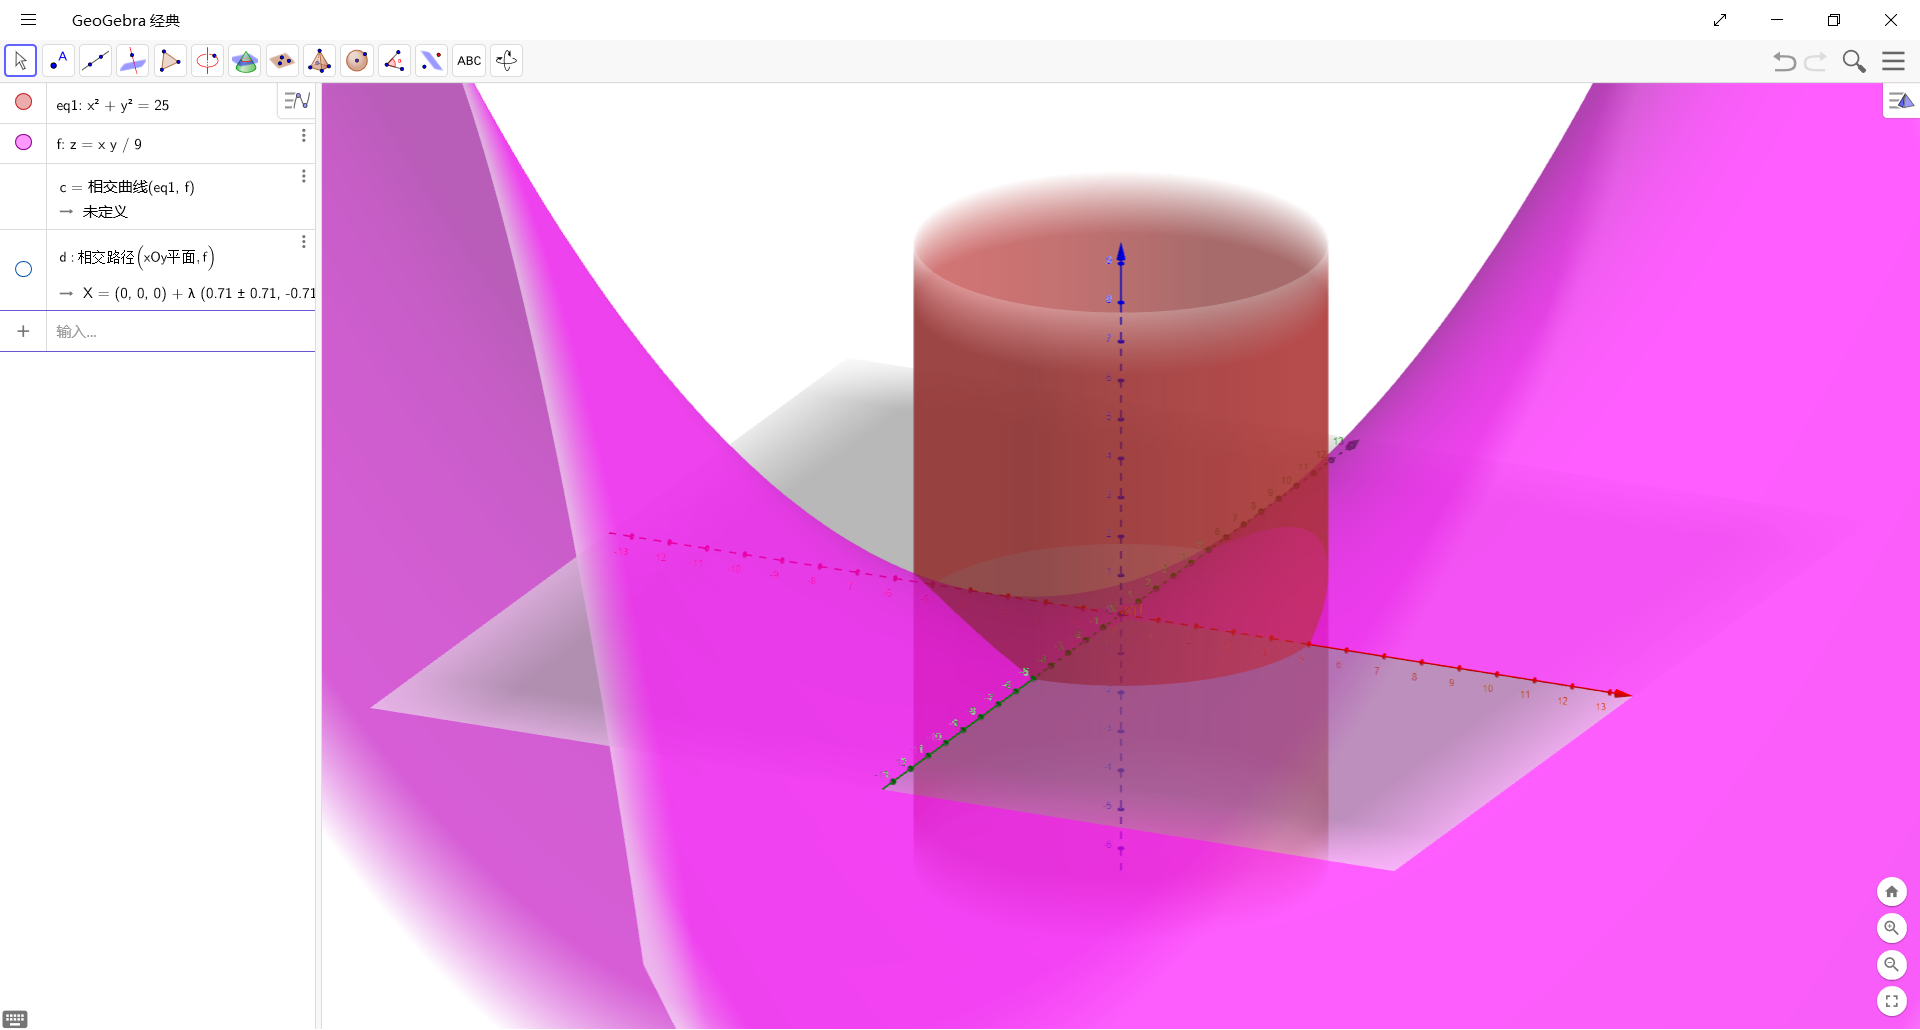
\includegraphics[scale=0.3]{交线.png}
                \caption{交线}
                \label{交线}
            \end{figure}
        \end{enumerate}
    \end{enumerate}



    \subsection{条件极值——(最)优化问题}
    \paragraph{\colorbox{lime}{定义}}设$\Omega\in\mathbb{R}^n$是一个区域,$\boldsymbol{x}_0\in\Omega,f(\boldsymbol{x})$是$\Omega$上的一个函数。如果$\exists r>0$s.t.$O(\boldsymbol{x}_0,r)\subset\Omega$,而且$f(\boldsymbol{x})\ge f(\boldsymbol{x}_0),\forall\boldsymbol{x}\in O(\boldsymbol{x}_0,r)$,则称$\boldsymbol{x}_0$是$f$在$\Omega$上的极小值点,$f(\boldsymbol{x}_0)$称为相应的极小值;如果“$f(\boldsymbol{x})\ge f(\boldsymbol{x}_0),\forall\boldsymbol{x}\in O(\boldsymbol{x}_0,r)$”换成"$f(\boldsymbol{x})> f(\boldsymbol{x}_0),\forall\boldsymbol{x}\in O(\boldsymbol{x}_0,r)\backslash\{\boldsymbol{x}_0\}$",则称$\boldsymbol{x}_0$为$f$在$\Omega$上的一个严格极小(大)值点,相应的$f(\boldsymbol{x}_0)$称为严格极小(大)值。“严格极小(大)值点”“严格极小(大)值”等定义类似。

    \paragraph{\textcolor{red}{Q:}}如何来求极值与极值点?\\
    先来看必要条件:

    回顾一元函数:\begin{enumerate}
        \item 若$f\in C^1(a,b),x_0\in(a,b)$是极值点,则$f'(x_0)=0$;
        \item 若$f\in C^2(a,b),x_0\in(a,b)$是极小值点,则$f''(x_0)\ge 0$;若$x_0$是极大值点,则$f''(x_0)\le 0$;
    \end{enumerate}

    \paragraph{\colorbox{lime}{定理}}($n$元函数取值的必要条件)  若$\Omega\subset\mathbb{R}^n$是一个区域,$\boldsymbol{x}_0\in\Omega,f\in C^1(\Omega)$
    \begin{enumerate}[(1)]
        \item 如果$\boldsymbol{x}_0$是$f$在$\Omega$上的一个极值点,则$\nabla f(\boldsymbol{x}_0)=0$(即$\p{f}{x_i}(\boldsymbol{x}_0)=0,i=1,2,\cdots,n$);
        \item 若$f\in C^2(\Omega),\boldsymbol{x}_0$是$f$在$\Omega$上的一个极大值点,则Hesse矩阵$Hf(\boldsymbol{x}_0)=\left(\frac{\partial^2f}{\partial x_i\partial x_j}(\boldsymbol{x}_0)\right)\le 0$,即$Hf(\boldsymbol{x}_0)$是半负定矩阵;反之若为极小值点,则$Hf(\boldsymbol{x}_0)\ge 0$,即$Hf(\boldsymbol{x}_0)$是半正定矩阵。
    \end{enumerate}
    \begin{proof}
        \textcolor{blue}{方法1:}令$g(t)=f(\boldsymbol{x}_0+t\boldsymbol{h})$,其中$|t|<\rho,\boldsymbol{h}\in S^{n-1}$(单位球面),则$g(t)\in C^1(-\rho,\rho)$,而且$g(t)\ge g(0),\forall t\in(-\rho,\rho)$,所以$g'(0)=0\Rightarrow \boldsymbol{h}\nabla f(\boldsymbol{x}_0)=0,\forall\boldsymbol{h}\in S^{n-1}$,从而$\nabla f(\boldsymbol{x}_0)=0$.

        若$f\in C^2(\Omega),$则$g\in C^2(-\rho,\rho)$;又当$\boldsymbol{x}_0$是$f$在$\Omega$上的极大值点时,$0$是$g$在$(-\rho,\rho)$上的极大值点,所以$g''(0)\le 0$。而
        $$g'(t)=\boldsymbol{h}\nabla f(\boldsymbol{x}_0+t\boldsymbol{h})=\sum_{i=1}^nh_i\p{f}{x_0}(\boldsymbol{x}_0+t\boldsymbol{h})$$
        $$g''(t)=\sum_{i=1}^nh_i\left(\sum_{j=1}^nh_j\frac{\partial^2f}{\partial x_i\partial x_j}(\boldsymbol{x}_0+t\boldsymbol{h})\right)=\sum_{i,j=1}^nh_ih_j\frac{\partial^2f}{\partial x_i\partial x_j}(\boldsymbol{x}_0+t\boldsymbol{h})$$
        所以$$g''(0)=\sum_{i,j=1}^nh_ih_j\frac{\partial^2f}{\partial x_i\partial x_j}(\boldsymbol{x}_0)=\boldsymbol{h}\cdot Hf(\boldsymbol{x}_0)\boldsymbol{h}^T\le 0,\forall\boldsymbol{h}\in S^{n-1}$$
        所以$Hf(\boldsymbol{x}_0)\le 0$.

        \textcolor{blue}{方法2:}若$\boldsymbol{x}_0$是$f$在$\Omega$上的一个极小值点,则$f(\boldsymbol{x}_0+\varepsilon\boldsymbol{h})\ge f(\boldsymbol{x}_0),\forall|\varepsilon|<\rho,\boldsymbol{h}\in S^{n-1}$。又因为
        $$f(\boldsymbol{x}_0+\varepsilon\boldsymbol{h})=f(\boldsymbol{x}_0)+\nabla f(\boldsymbol{x}_0)\cdot\varepsilon\boldsymbol{h}+\frac{1}{2}(\varepsilon\boldsymbol{h})Hf(\boldsymbol{x}_0)(\varepsilon\boldsymbol{h})^T+o(\varepsilon^2)=f(\boldsymbol{x}_0)+\frac{\varepsilon^2}{2}\boldsymbol{h}Hf(\boldsymbol{x}_0)\boldsymbol{h}^T+o(\varepsilon^2)$$
        我们有
        $$\frac{\varepsilon^2}{2}\boldsymbol{h}Hf(\boldsymbol{x}_0)\boldsymbol{h}^T+o(\varepsilon^2)\ge 0,\forall|\varepsilon|<\rho,
        boldsymbol{h}\in S^{n-1}$$
        $$Rightarrow\frac{1}{2}\boldsymbol{h}Hf(\boldsymbol{x}_0)\boldsymbol{h}^T+\frac{o(\varepsilon^2)}{\varepsilon^2}\ge 0,\forall\boldsymbol{h}\in S^{n-1}$$
        令$\varepsilon\to 0$,得$\boldsymbol{h}Hf(\boldsymbol{x}_0)\boldsymbol{h}^T\ge 0,\forall\boldsymbol{h}\in S^{n-1},$所以$Hf(\boldsymbol{x}_0)\ge 0$.
    \end{proof}

    \paragraph{\colorbox{pink}{例}}若$\begin{cases}
        \frac{\partial^2f}{\partial x^2}+\frac{\partial^2f}{\partial y^2}-f=0,x^2+y^2<1,\\
        f|_{x^2+y^2=1}=0
    \end{cases}$,则$f\equiv 0$.
    \begin{proof}
        令$\Omega=\{(x,y):x^2+y^2<1\}$.若$\exists(x_0,y_0)\in \Omega,s.t.f(x_0,y_0)=\max_{\Omega}|f|>0$,则$$\begin{pmatrix}
            \frac{\partial^2f}{\partial x^2}&\frac{\partial^2f}{\partial x\partial y}\\
            \frac{\partial^2f}{\partial x\partial y}&\frac{\partial^2f}{\partial y^2}
        \end{pmatrix}(x_0,y_0)\le 0\Rightarrow \left(\frac{\partial^2f}{\partial x^2}+\frac{\partial^2f}{\partial y^2}\right)(x_0,y_0)\le 0$$
        从而$\left(\frac{\partial^2f}{\partial x^2}+\frac{\partial^2f}{\partial y^2}\right)(x_0,y_0)-f(x_0,y_0)<0$,矛盾。
    \end{proof}

    \paragraph{\colorbox{orange!75}{Note}}\begin{enumerate}
        \item 只是必要条件。例:$f(x,y)=xy$(图像见\ref{xy}),则$\nabla f(0,0)=(0,0)$,但是$(0,0)$不是$f$的极值点。又例:$f(x,y)=x^3+y^3$(图像见\ref{x^3+y^3}),则$\nabla f(0,0)=(0,0),Hf(0,0)=\begin{pmatrix}
            0&0\\
            0&0
        \end{pmatrix}$,但$(0,0)$不是极值点。例:$f(x,y)=4xy^2+x^2+y^4$(图像见\ref{4xy^2+x^2+y^4}),此时有$\nabla f(0,0)=(0,0),Hf(0,0)=\begin{pmatrix}
            2&0\\
            0&0
        \end{pmatrix}\ge 0$,但是$(0,0)$不是极值点。

        \begin{figure}[h!t!b!p]
            \centering
            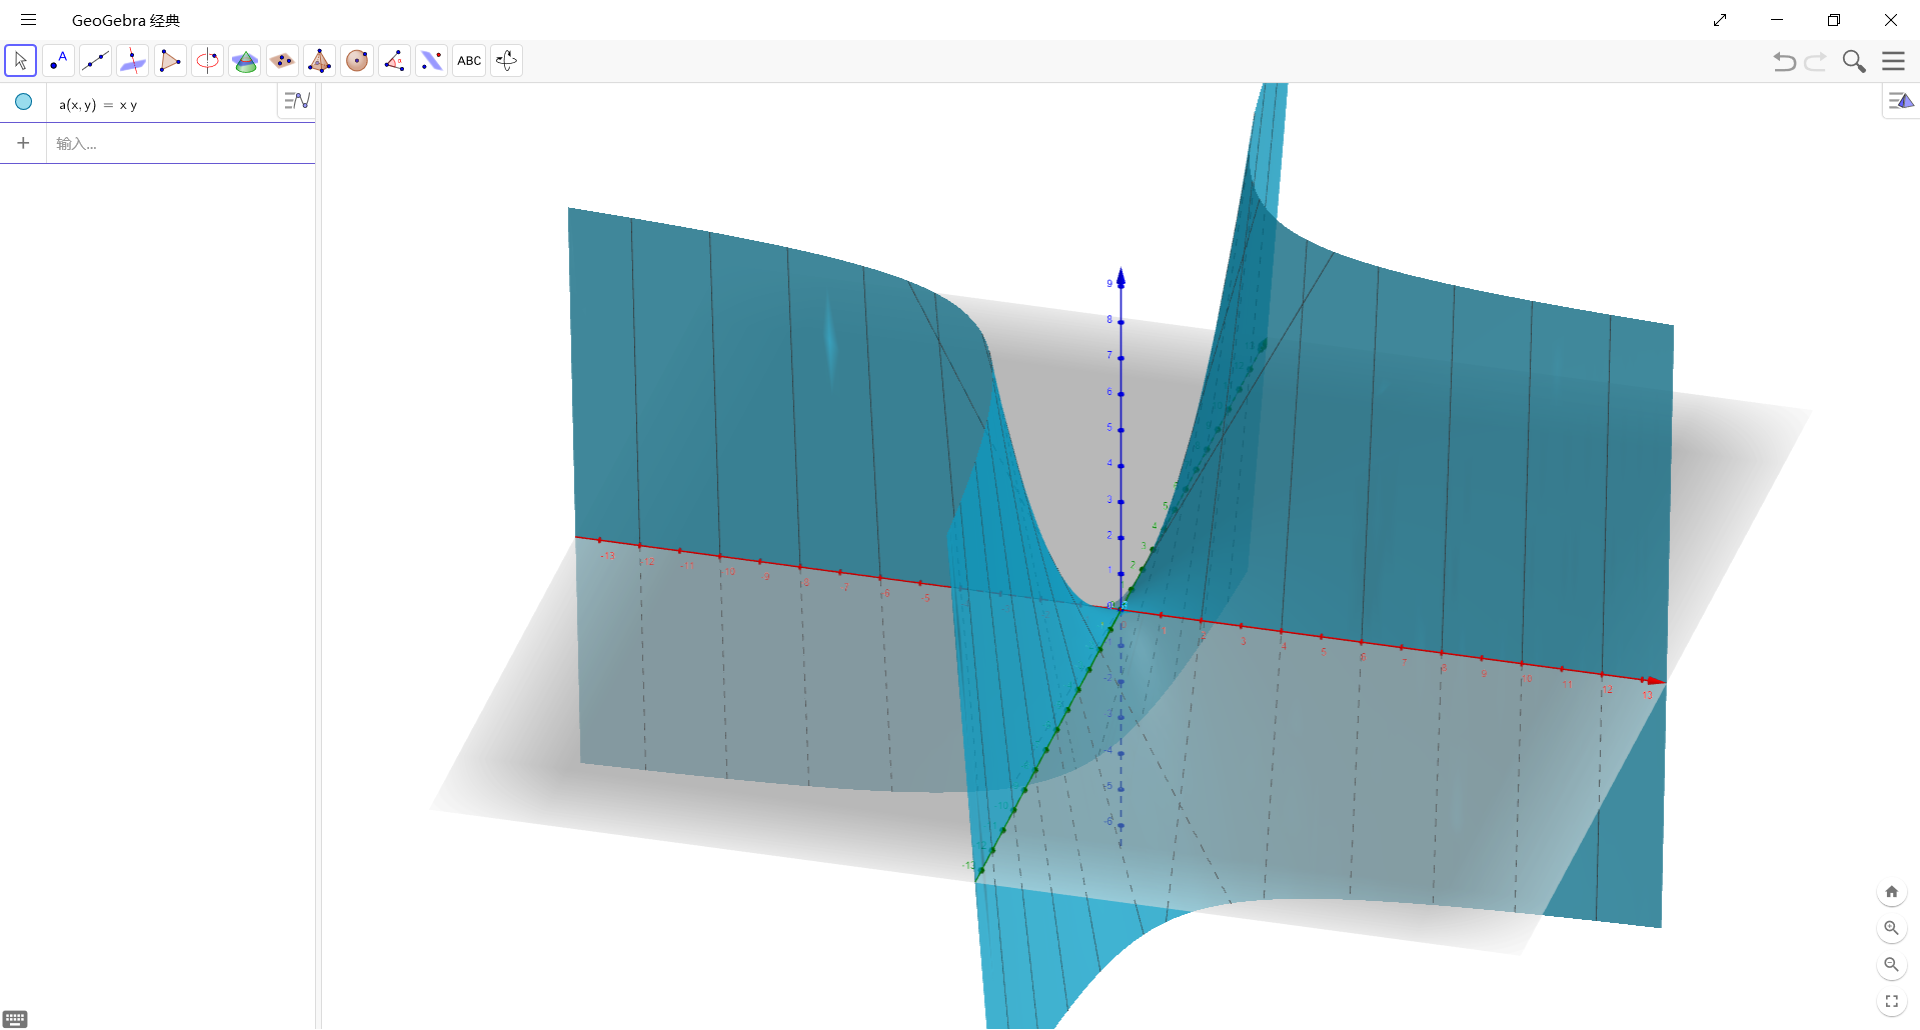
\includegraphics[scale=0.3]{z=xy.png}
            \caption{$f(x,y)=xy$}
            \label{xy}
        \end{figure}

        \begin{figure}[h!t!b!p]
            \centering
            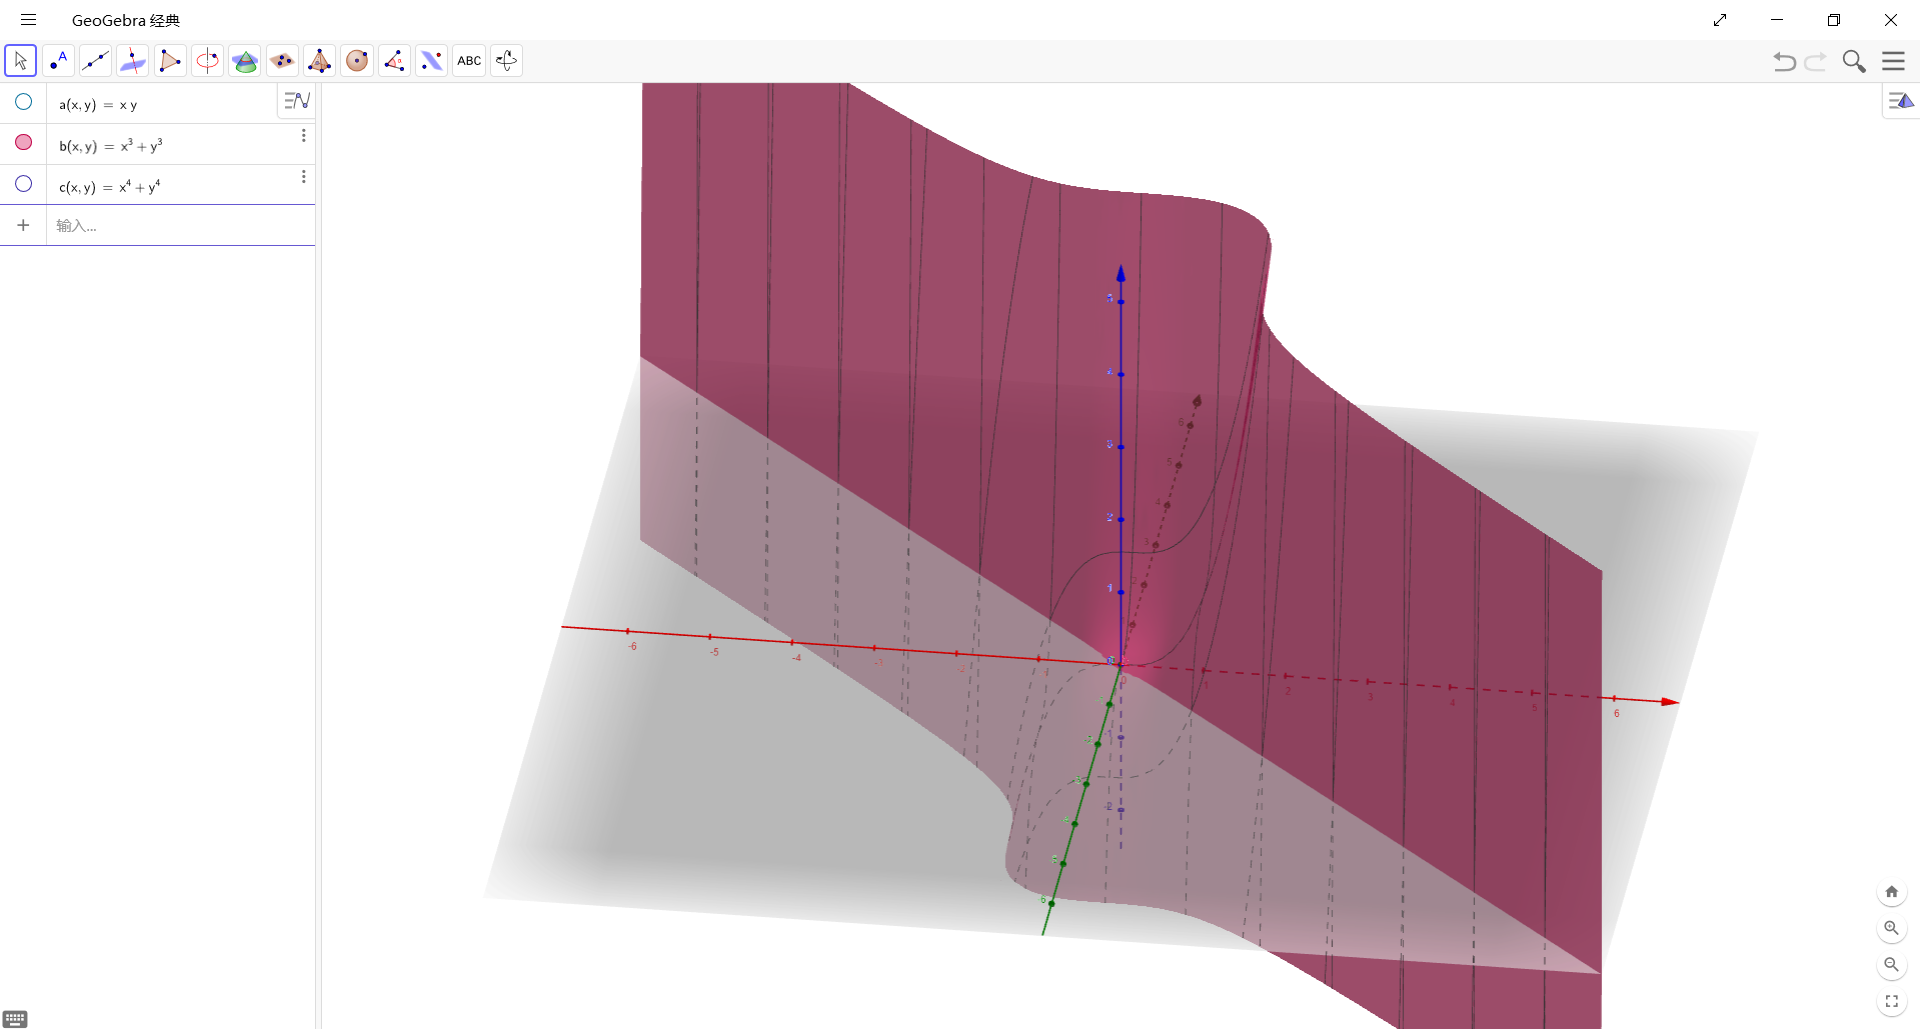
\includegraphics[scale=0.3]{z=x^3+y^3.png}
            \caption{$f(x,y)=x^3+y^3$}
            \label{x^3+y^3}
        \end{figure}

        \begin{figure}[h!t!b!p]
            \centering
            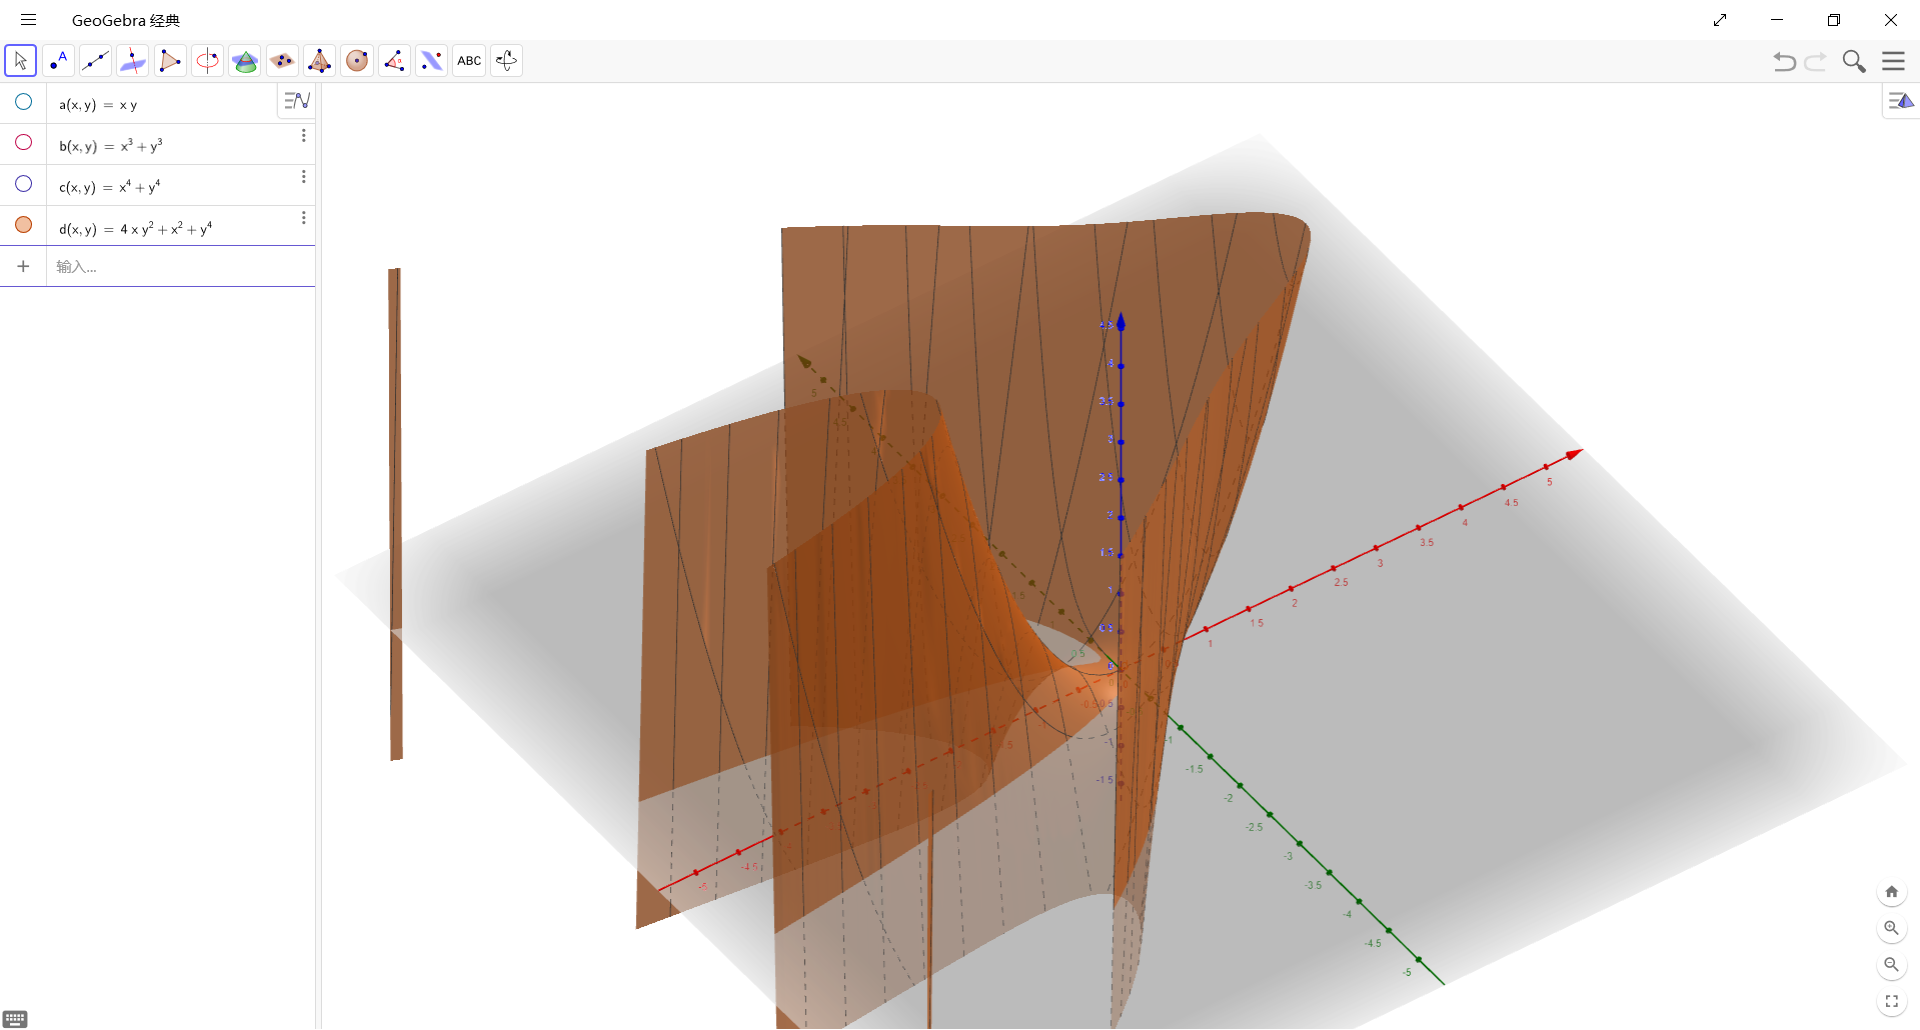
\includegraphics[scale=0.3]{4xy^2+x^2+y^4.png}
            \caption{$f(x,y)=4xy^2+x^2+y^4$}
            \label{4xy^2+x^2+y^4}
        \end{figure}

        \item 偏导数不存在的点又可能是极值点。例:$f(x,y)=|x|+|y|$(图像参考\ref{abs(x)+abs(y)}),$(0,0)$为其极小值,但$f$在$(0,0)$处偏导数不存在。
        \begin{figure}[h!t!b!p]
            \centering
            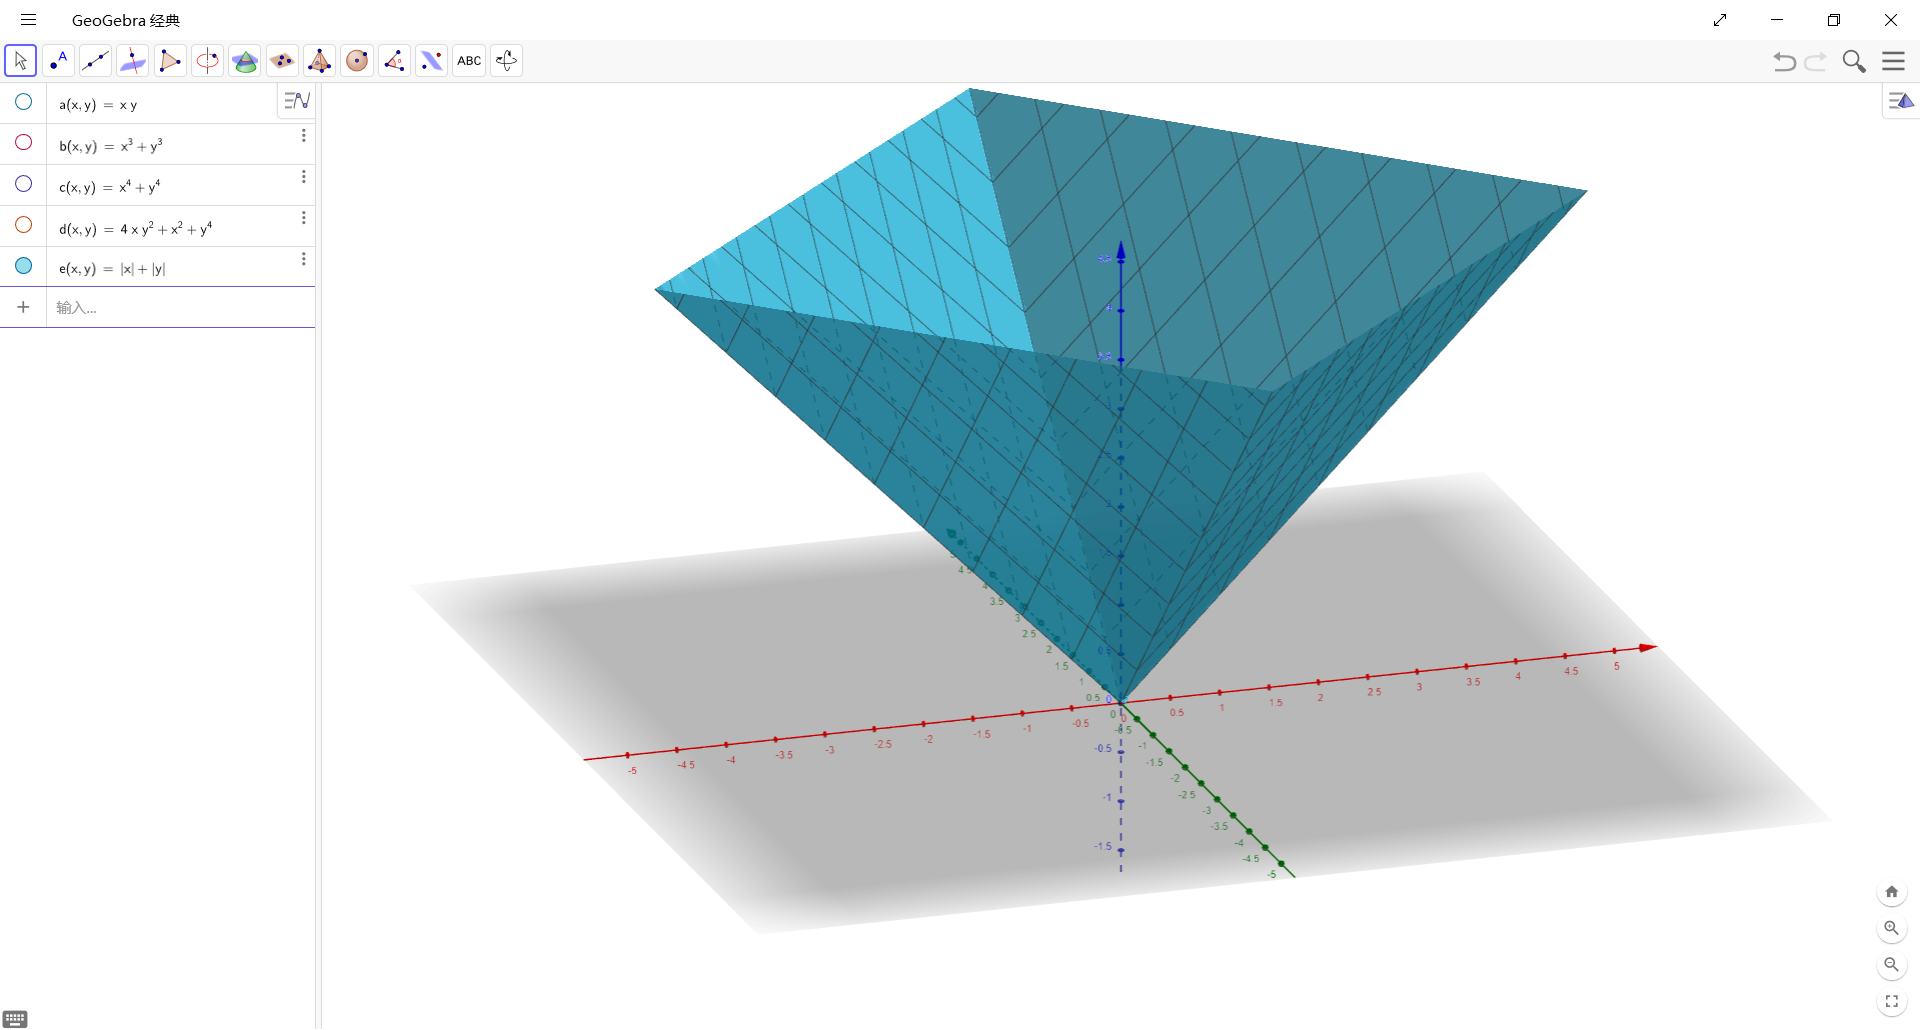
\includegraphics[scale=0.3]{z=abs(x)+abs(y).png}
            \caption{$f(x,y)=|x|+|y|$}
            \label{abs(x)+abs(y)}
        \end{figure}
    \end{enumerate}
\end{document}